\documentclass[aspectratio=169,handout,10pt]{beamer}
\usepackage[italian]{babel}
\usepackage{animate}
\usepackage{amsmath}
\usepackage[makeroom]{cancel}
\usepackage{sourcecodepro}
\usepackage{xcolor}
\usepackage{xparse}
\usepackage{listings}
\usepackage{float}
\usepackage{color}
\usepackage{multicol}
\usepackage{tikz}
\usepackage{tikzscale}
\usepackage{makecell}
\usepackage{keystroke}
\usepackage{gitdags}
\usepackage{gitobject}

\usetikzlibrary{fadings}
\usetikzlibrary{patterns}
\usetikzlibrary{shadows.blur}
\usetikzlibrary{shapes}
\usetikzlibrary{fit}
\usetikzlibrary{positioning}
\usetikzlibrary{matrix}
\usetikzlibrary {shapes.symbols}

\newcommand{\quotebox}[1]{\begin{center}\fcolorbox{white}{blue!15!gray!15}{\begin{minipage}{0.9\linewidth}\vspace{10pt}\center\begin{minipage}{0.8\linewidth}{\space\Huge``}{#1}{\hspace{1.5em}\break\null\Huge\hfill''}\end{minipage}\smallbreak\end{minipage}}\end{center}}

\usetheme{Rochester}


\definecolor{codegreen}{rgb}{0,0.6,0}
\definecolor{codegray}{rgb}{0.5,0.5,0.5}
\definecolor{codepurple}{rgb}{0.58,0,0.82}
\definecolor{backcolour}{rgb}{0.95,0.95,0.92}
 
\newfontfamily\Lato[Ligatures=TeX]{Lato}

\usefonttheme{professionalfonts}

\setsansfont{Lato}[
  UprightFont=*-Light,
  ItalicFont=*-LightItalic,
  BoldFont=*-Regular,
  BoldItalicFont=*-Italic
]

\lstset{backgroundcolor=\color{backcolour},   
    commentstyle=\color{codegreen},
    keywordstyle=\color{blue},
    numberstyle=\tiny\color{codegray},
    stringstyle=\color{codepurple},
    keepspaces=true,                 
    numbersep=5pt,                  
    showspaces=false,                
    showstringspaces=false,
    breaklines=true,
    showtabs=false,                  
    tabsize=2,basicstyle=\ttfamily}


\renewcommand{\CancelColor}{\color{red}}



\title{Alla scoperta di Git}

\titlegraphic{
\includegraphics[width=.45\textwidth]{media/Git-logo.pdf}}


\begin{document}

\AtBeginSection[]
{
    \begin{frame}
        \begin{multicols}{2}
            \tableofcontents[currentsection,hideothersubsections]
        \end{multicols}
    \end{frame}
}


\begin{frame}
    \maketitle
\end{frame}

\section{Le 5 W}

\begin{frame}{Cos'è Git}
    \begin{itemize}
        \item Git è un software di controllo di versione \textbf{distribuito} (DVCS - Distributed Version Control System).
        \item Permette di tenere traccia delle modifiche apportate ai file di un progetto nel tempo.
        \item È stato creato da Linus Torvalds nel 2005 per gestire lo sviluppo del kernel Linux.
    \end{itemize}
\end{frame}
\begin{frame}{Cosa fa Git}
    \begin{itemize}
        \item Git si occupa di archiviare la cronologia delle modifiche al progetto.
        \item Vengono registrate tutte le modifiche, si può tornare indietro e si può confrontare il codice.
        \item Le modifiche al progetto restano in locale e non vengono sincronizzate in realtime: bisogna effettuare un \textbf{commit}, che contiene una descrizione sintetica delle modifiche (il commit message) e le informazioni sull'autore.
        \item Ogni \textbf{commit} rappresenta uno stato del progetto in un determinato momento.
        \item Un \textbf{commit} rappresenta l'unità minima logica di un cambiamento.
        \item I commit sono organizzati in una history (o log) dei cambiamenti.
        \item Git permette di gestire più branch di sviluppo, per esempio per feature diverse o team separati.
        \item Git utilizza un sistema di branching e merging per gestire le diverse linee di sviluppo.
        \item Git ti permette di scoprire chi ha effettuato delle modifiche e perché.
    \end{itemize}
\end{frame}
\begin{frame}{Quando si usa Git}
    \begin{itemize}
        \item Git si utilizza su un \textbf{progetto}, cioè il codice per una app o un software o un suo componente, possiamo individuare un progetto come una struttura di cartelle o ``file tree''.
        \item Uno sviluppatore del team potrebbe lavorare su una nuova funzionalità del progetto mentre un altro sviluppatore corregge un bug non correlato modificando il codice, ogni sviluppatore può apportare le proprie modifiche in diverse parti del file tree.
        \item Il controllo della versione aiuta i team a risolvere questo tipo di problemi, aumentando le capacità di sviluppo contemporaneo e simultaneo, riducendo i conflitti e avendo uno storico delle modifiche.
    \end{itemize}
\end{frame}
\begin{frame}{Dove si usa Git}
    \begin{itemize}
        \item Git si utilizza su qualsiasi computer, su qualsiasi tipo di file (anche se Git preferisce i file di testo) e su progetti di qualsiasi dimensione.
        \item Non vi sono particolari limiti all'utilizzo.
        \item Git si utilizza quando è necessario condividere il codice con altri device o altre persone, perché rende la condivisione molto semplice.
        \item Sebbene sia possibile sviluppare software senza utilizzare alcun controllo di versione, ciò comporta un enorme rischio per il progetto che nessun team di professionisti dovrebbe accettare. Quindi la domanda non è se usare il controllo versione ma quale sistema di controllo versione usare (VCS).
    \end{itemize}
\end{frame}
\begin{frame}{Perché si usa Git}
    \begin{itemize}
        \item Git ti permette di ripristinare i file alle versioni precedenti per rimuovere modifiche errate o non volute
        \item Git ti permette di vedere la cronologia delle modifiche ai file e quindi raccoglie le conoscenze del team sullo sviluppo, magari è stata modificata una funzione perché ha un bug, ma data la memoria corta viene rifatto il codice uguale a prima, dimenticandosi dell'altro bug.
        \item Il controllo della versione protegge il codice sorgente sia dalla catastrofe sia dal degrado casuale dell'errore umano e delle conseguenze indesiderate.
        \item Gli sviluppatori di software che lavorano in team scrivono continuamente nuovo codice sorgente e modificano il codice sorgente esistente: magari il codice non è perfettamente aggiornato o dopo una semplice modifica tutti gli sviluppatori non riescono più a compilare.
        \item Git ti permette di effettuare operazioni di \textbf{merge} tra i vari branch del progetto segnalando e gestendo eventuali \textbf{conflitti}.
    \end{itemize}
\end{frame}
\begin{frame}{Perché imparare Git quando posso giocare con i nomi dei file?}
    \begin{minipage}{0.7\textwidth}
        \begin{figure}
            \includegraphics{media/def_def_def.tikz}
        \end{figure}
    \end{minipage}%
    \begin{minipage}{0.3\textwidth}
        Ecco un esempio pratico per cui è meglio un repository Git: come si fa a sapere qual è l'ultimo file, quello definitivo?
    \end{minipage}
\end{frame}
\begin{frame}
    \quotebox{Un bug non è mai solo un errore. Rappresenta qualcosa di più. Un errore nel modo di pensare. Perché, fuori dallo schermo, la vita è piena di bug e ti rende come sei. Il bug costringe il software ad adattarsi, per causa sua deve evolvere in qualcosa di nuovo. Deve aggirare l'ostacolo o superarlo. Qualsiasi cosa accada si trasforma. Diventa qualcosa di nuovo. La versione successiva. L'inevitabile upgrade. Mr. Robot - Elliot}
\end{frame}
\begin{frame}{Best practice}
    \begin{description}
        \item[Fare spesso commit] I commit sono facili e veloci. Dovrebbero essere eseguiti frequentemente per acquisire gli aggiornamenti di una base di codice. Ogni commit è uno snapshot su cui è possibile ripristinare la codebase se necessario. I commit frequenti offrono molte opportunità di ripristinare o annullare il lavoro. Un gruppo di commit può essere combinato in un singolo commit (squash) usando un rebase per avere una history più pulita.
        \item[Programma sempre sulla versione corretta] i VCS permettono aggiornamenti rapidi da più sviluppatori. È facile avere una copia locale non sincronizzata, rendendo più difficile il merge!
        \item[Dettaglia bene le modifiche] Ogni commit ha un commit message. È importante scrivere commit message chiari e descrittivi: una prima riga breve che riassume la modifica e, se serve, una descrizione più lunga del perché.
    \end{description}
\end{frame}
\begin{frame}{Best practice}
    \begin{description}
        \item[Usa i branch] Il branch è un potente meccanismo del VCS che consente agli sviluppatori di creare una linea di sviluppo separata. I branch dovrebbero essere usati frequentemente in quanto sono rapidi ed economici.
        \item[Concorda un workflow unico] Si decidono delle linee guida per i merge, per la creazione e il naming dei branch, per le pull request e così via!
        \item[Un commit, una modifica logica] I commit rappresentano l'unità minima logica di un cambiamento: frequenti sì, ma ognuno deve avere senso da solo (niente ``fix'', ``fix 2'', ``ora va'').
    \end{description}
\end{frame}

\section{Come funziona un DVCS come Git}

\begin{frame}{DVCS}{Distributed Version Control Systems}
    \begin{minipage}{0.6\textwidth}
        \begin{figure}
            \includegraphics{media/dvcs.tikz}
        \end{figure}
    \end{minipage}%
    \begin{minipage}{0.4\textwidth}
        Nei Distributed Version Control Systems i client non scaricano solo la versione più recente dei file, ma fanno una copia completa del repository, history compresa.
    \end{minipage}
\end{frame}
\begin{frame}{DVCS}{Distributed Version Control Systems}
    \begin{minipage}{0.6\textwidth}
        \begin{figure}
            \includegraphics{media/dvcs.tikz}
        \end{figure}
    \end{minipage}%
    \begin{minipage}{0.4\textwidth}
        Nei Distributed Version Control Systems ci sono due operazioni principali:
        \begin{description}
            \item[Pull] per scaricare le modifiche dal server centrale
            \item[Push] per caricare le modifiche sul server centrale
        \end{description}
        Queste operazioni vengono effettuate su uno o più server che contengono il \textbf{repository remoto}, l'indirizzo del repository viene comunemente chiamato \textbf{Remote URL}.
    \end{minipage}
\end{frame}

\section{Architettura di Git}

\begin{frame}{Design di Git}
    Il design di Git è stato basato su 5 punti:
    \begin{itemize}
        \item Velocità
        \item Semplicità di design e uso
        \item Supporto per sviluppo non lineare (migliaia di versioni parallele)
        \item Completamente distribuito
        \item Abilità di gestire grandi progetti
    \end{itemize}
    
    La differenza principale tra Git e altri VCS sta in come Git pensa e
    vede i propri dati.
    
    \begin{itemize}
        \item Molti VCS (come CVS e Subversion) vedono i dati che gestiscono come un set di file e di cambiamenti apportati a tali file nel tempo (delta-based version control)
        \item Git vede i dati come una serie di snapshot di un filesystem in miniatura (e poi comprime gli oggetti simili nei packfile usando i delta).
    \end{itemize}
\end{frame}
\begin{frame}{Gli oggetti di Git}
    Git è basato principalmente su due strutture dati:
    \begin{itemize}
        \item Un \textbf{index mutabile} (chiamato anche staging area o cache) nel quale vengono raccolte le informazioni sulla working directory
        \item Un \textbf{object database immutabile} che può contenere 4 tipi di oggetti (blob, tree, commit, tag), queste strutture possono essere viste come dei \textbf{puntatori}.
    \end{itemize}    
\end{frame}
\begin{frame}{Gli oggetti di Git}{blob}
    \begin{minipage}{0.5\textwidth}
        Un \textbf{blob} (Binary Large Object) rappresenta il contenuto di un file. Ciascun blob all'interno dell'object database di Git è identificato dal proprio hash (SHA-1 di default; SHA-256 è supportato con \texttt{git init --object-format=sha256}).
    \end{minipage}%
    \begin{minipage}{0.5\textwidth}
        \begin{figure}
            \includegraphics{media/architettura_git_blob.tikz}
        \end{figure}
    \end{minipage}
\end{frame}
\begin{frame}{Gli oggetti di Git}{tree}
    \begin{minipage}{0.5\textwidth}
        Un \textbf{tree} è l'equivalente di una directory; contiene una lista di nomi di file e il riferimento al relativo oggetto, sia esso un file, un link simbolico o una directory.
    \end{minipage}%
    \begin{minipage}{0.5\textwidth}
        \begin{figure}
            \scalebox{0.5}{
                \includegraphics[width=1.3*\textwidth]{media/architettura_git_tree.tikz}
            }
        \end{figure}
    \end{minipage}
\end{frame}
\begin{frame}{Gli oggetti di Git}{commit object}
    \begin{minipage}{0.35\textwidth}
        Un \textbf{commit object} è un oggetto che collega vari tree object formando una storia; contiene l'hash del tree object, un timestamp, il commit message, nome ed email di autore e committer e il riferimento ai commit genitori (nessuno per il primo commit, due o più per un merge).

        Un commit object è identificato da un hash, per esempio \texttt{2c7ae1b9865e58797ba326d2f7a115bebb034fd7}. Il riferimento al commit corrente (di solito tramite il branch corrente) si chiama \texttt{HEAD}.
    \end{minipage}%
    \begin{minipage}{0.65\textwidth}
        \begin{figure}
            \scalebox{0.5}{
                \includegraphics[width=2*\textwidth]{media/architettura_git.tikz}
            }
        \end{figure}
    \end{minipage} 
\end{frame}
\begin{frame}{Gli oggetti di Git}{tag}
    \begin{minipage}{0.4\textwidth}
        Un \textbf{tag} contiene un puntatore ad un qualsiasi altro oggetto presente nel database e i suoi metadati
    \end{minipage}%
    \begin{minipage}{0.6\textwidth}
        \begin{figure}
            \scalebox{0.75}{
                \includegraphics[width=1.33*\textwidth]{media/architettura_git_tag.tikz}
            }
        \end{figure}
    \end{minipage} 
\end{frame}

\section{Storia di Git e differenze con altri DVCS}

\begin{frame}{Storia di Git}
    Git è nato nel 2005 per gestire il codice sorgente del kernel Linux.

    Scritto da Linus Torvalds, che voleva un sistema distribuito che si potesse usare come BitKeeper, ma nessuno dei sistemi disponibili gratuitamente soddisfaceva i suoi bisogni, particolarmente il suo bisogno di velocità. BitKeeper non lo si poteva più usare gratuitamente in quanto Andrew Tridgell aveva effettuato il reverse engineering dei protocolli. Dal 2005 Git è mantenuto da Junio Hamano.
    
    È un sistema di version control distribuito, pensato per gestire grandi cartelle di codice sorgente ma con la possibilità di gestire qualsiasi tipo di file.
\end{frame}
\begin{frame}{Il nome Git}
    Cosa può significare Git?
    \begin{enumerate}
        \item 3 lettere casuali mai usate dagli OS UNIX quindi utilizzabili.
        \item nello slang americano significa idiota/stupido
        \item Global Information Tracker ma solo quando sei bravo (monitoraggio delle informazioni globali)
        \item Goddamn Idiotic Truckload (dannato carico di camion idiota) ma solo quando non funziona
    \end{enumerate}
    Linus affermò di aver scelto Git proprio perché nello slang americano significa idiota/stupido e gli sembrava divertente.
\end{frame}

\begin{frame}{Come scegliere un VCS}
    Cosa deve avere un VCS perché sia valido?
    \begin{enumerate}
        \item \textbf{Una cronologia completa delle modifiche a lungo termine di ogni file.} Deve poter memorizzare tutti i cambiamenti apportati da molte persone nel corso degli anni. Le modifiche includono la creazione e la cancellazione di file, nonché modifiche al loro contenuto. Questa cronologia dovrebbe includere anche l'autore, la data e le note scritte sullo scopo di ogni modifica. Avere la cronologia completa consente di tornare alle versioni precedenti per aiutare nell'analisi della causa principale dei bug ed è fondamentale quando è necessario risolvere i problemi nelle versioni precedenti del software. Se il software viene lavorato attivamente, quasi tutto può essere considerato una ``versione precedente'' del software.
        \item \textbf{Branching e merging.} La creazione di branch permette ai membri del team di lavorare contemporaneamente senza intralciarsi a vicenda; ogni volta che un pezzo di codice è completato si fa il merge, e chi lo fa deve gestire solamente i veri conflitti, senza dover controllare tutti i file anche per minuscole differenze.
    \end{enumerate}
\end{frame}
\begin{frame}{Come scegliere un VCS}
    \begin{enumerate}\setcounter{enumi}{2}
        \item \textbf{Tracciabilità.} Essere in grado di tracciare ogni modifica apportata al software e essere in grado di annotare ogni modifica con un messaggio che descrive lo scopo e l'intento della modifica può aiutare l'analisi della causa principale del bug. Avere la cronologia annotata del codice a portata di mano quando si legge il codice, cercando di capire cosa sta facendo e perché è così progettato può consentire agli sviluppatori di apportare modifiche corrette e armoniose in accordo con il progetto a lungo termine previsto del sistema. Ciò può essere particolarmente importante per lavorare in modo efficace con il codice legacy ed è cruciale per consentire agli sviluppatori di stimare il lavoro futuro con precisione.      
    \end{enumerate}
\end{frame}
\begin{frame}{Differenze e Snapshot}
    \begin{columns}
        \begin{column}{0.5\textwidth}
            \textbf{Snapshot} Ogni volta che si salva lo stato di un progetto viene fatto uno snapshot di tutti i file e salvato nel VCS
            
            \scalebox{0.66}{
                \includegraphics[width=1.5*\textwidth]{media/snapshot.tikz}
            }
        \end{column}
        \begin{column}{0.5\textwidth}
            
            \textbf{Differenze} Ogni volta che si salva lo stato di un progetto vengono salvate nel VCS le differenze (delta) rispetto alla versione precedente
            
            \scalebox{0.66}{
                \includegraphics[width=1.5*\textwidth]{media/diff.tikz}
            }
        \end{column}
    \end{columns}
\end{frame}

\begin{frame}{Git e Subversion}
    \begin{columns}
        \begin{column}{0.5\textwidth}
            \textbf{Git}  è un DVCS creato da Linus Torvalds nel 2005 per semplificare la gestione del repository del kernel Linux.
            
            Utilizza le snapshot per salvare le modifiche.
            
            
        \end{column}
        \begin{column}{0.5\textwidth}
            
            \textbf{S}ub\textbf{V}ersio\textbf{N} è un VCS centralizzato creato per sostituire CVS, ritenuto ormai obsoleto.
            
            Utilizza le differenze per salvare le modifiche.
            
            
            
        \end{column}
    \end{columns}
\end{frame}

\begin{frame}{Git e Subversion}
    \begin{columns}
        \begin{column}{0.5\textwidth}
            \textbf{Git}
            \begin{itemize}
                \item Distribuito
                \item Copia locale completa del repository dove lavorare
                \item Non si può limitare l'accesso a singole directory: si dà accesso all'intero repository
                \item Cronologia delle modifiche disponibili anche offline
                \item Connessione di rete necessaria solo alla sincronizzazione
            \end{itemize}
            
            
        \end{column}
        \begin{column}{0.5\textwidth}
            
            \textbf{S}ub\textbf{V}ersio\textbf{N} 
            \begin{itemize}
                \item Centrale
                \item Copia locale dell'ultima versione dove lavorare
                \item Si può limitare l'accesso a singole directory (path-based authorization)
                \item Cronologia delle modifiche non disponibile offline
                \item Connessione di rete sempre necessaria
            \end{itemize}
            
            
        \end{column}
    \end{columns}
\end{frame}

\begin{frame}[fragile]{Git e Subversion}
    \begin{columns}
        \begin{column}{0.5\textwidth}
            \textbf{Git}
            \begin{itemize}
                \item Git non traccia esplicitamente i rename: per seguire la history di un file rinominato serve \lstinline{git log --follow}
                \item Supporto a repository enormi tramite partial clone, sparse-checkout e Scalar
                \item Git non adora i file binari, per quelli grandi c'è Git LFS
                \item Esistono molti hosting Git gratuiti tra cui GitHub, GitLab e Bitbucket
                      
            \end{itemize}
            
            
        \end{column}
        \begin{column}{0.5\textwidth}
            
            \textbf{S}ub\textbf{V}ersio\textbf{N} 
            \begin{itemize}
                \item Nonostante non sia un sistema distribuito è facile fare copie di backup 
                \item Pochi comandi, semplici e intuitivi
                \item Impossibile fare una copia locale se non puoi accedere al server Subversion
                \item Gli hosting Subversion gratuiti sono sempre più rari: GitHub ha rimosso il supporto a Subversion a gennaio 2024
                      
            \end{itemize}
            
            
        \end{column}
    \end{columns}
\end{frame}

\begin{frame}<presentation:0>{Git e Subversion}
    \framesubtitle{i numeri}
    N.B. dati non aggiornati
    \begin{table}
        \begin{tabular}{|p{0.30\textwidth}|p{0.30\textwidth}|p{0.30\textwidth}|}
            \hline & Subversion & Git \\
            \hline Data Source & \url{https://core.svn.wordpress.org/} & \url{https://github.com/wordpress/wordpress} \\
            \hline Numero di Revisioni & 42704 & 38070 \\
            \hline Dimensione del repository  & 195,153,948 bytes & 177,922,471 bytes \\
            \hline Software Version & Subversion 1.9.2, 64 bit & Git 2.6.3, 64 bit \\
            \hline Commento & Il repository è il dump  del repository ufficiale  di wordpress & Il repository viene mantenuto da GitHub, alcune revisioni vengono omesse \\
            \hline
        \end{tabular}
    \end{table}
\end{frame}

\begin{frame}<presentation:0>{Git e Subversion}
    \framesubtitle{dove non usarli}
    \begin{columns}
        \begin{column}{0.5\textwidth}
            \textbf{Git}
            \begin{itemize}
                \item L'utilizzo di Git è sconsigliato in progetti di medie/grandi dimensioni in quanto le principali operazioni diventano molto più lente    
            \end{itemize}            
        \end{column}
        \begin{column}{0.5\textwidth}
            \textbf{S}ub\textbf{v}ersio\textbf{n} 
            \begin{itemize}
                \item L'utilizzo di Subversion è sconsigliato nei progetti dove ci sono molte modifiche in parallelo sugli stessi file in quanto può avere solo una singola cronologia lineare e confonderlo è molto facile
            \end{itemize}
        \end{column}
    \end{columns}
\end{frame}

\begin{frame}[fragile]{Estensioni e altri DVCS}
    \begin{columns}
        \begin{column}{0.5\textwidth}
            \textbf{Git+Subversion}
            \begin{itemize}
                \item \texttt{git svn} permette di usare in maniera bidirezionale un repository Subversion da Git, con i vantaggi (e gli svantaggi) di entrambi
            \end{itemize}
            \textbf{Scalar}
            \begin{itemize}
                \item Nato in Microsoft come evoluzione di GVFS (VFS for Git, ora archiviato), dal 2022 è incluso in Git (\lstinline{scalar clone}) e configura partial clone, sparse-checkout e manutenzione in background per gestire repository enormi.
            \end{itemize}
        \end{column}
        \begin{column}{0.5\textwidth}
            \textbf{Mercurial}
            \begin{itemize}
                \item Mercurial è un'alternativa a Git e Subversion.
                \item Utilizza un sistema ibrido per il salvataggio degli stati:
                \item Utilizza un algoritmo di delta quando le differenze sono poche, altrimenti uno snapshot.
                \item Oggi è molto meno diffuso: Bitbucket ne ha rimosso il supporto nel 2020.
            \end{itemize}
        \end{column}
    \end{columns}
\end{frame}

\begin{frame}{Git e Subversion}
    \begin{figure}
\includegraphics[width=0.5\textwidth]{media/git-svn-copy.jpeg}\end{figure}
\end{frame}

\section{Installazione di Git}

\begin{frame}[fragile]{Installazione di Git su Linux}
    
    Per installare Git su Ubuntu, Debian, ... (su Fedora \lstinline{sudo dnf install git}, su Arch \lstinline{sudo pacman -S git})
    \begin{lstlisting}[language=bash]
$ sudo apt update
$ sudo apt install git\end{lstlisting}
    Dopodiché dal terminale verificare che l'installazione è andata a buon fine:
    \begin{lstlisting}[language=bash]
$ git --version\end{lstlisting}
    Impostiamo le nostre credenziali:
    \begin{lstlisting}[language=bash]
$ git config --global user.name "Emma Paris"
$ git config --global user.email "eparis@atlassian.com"\end{lstlisting}
    
    Consiglio di usare un nome e un'email che identifichino chiaramente chi ha scritto il codice (non furbissimo@gmail.com), perché restano salvati per sempre nella history, come in una blockchain o nella cronologia di Wikipedia.
\end{frame}
\begin{frame}[fragile]{Installazione di Git su Windows}
    Scarica da qui l'ultima versione: \url{https://gitforwindows.org/} oppure usa winget:
    \begin{lstlisting}
winget install --id Git.Git -e\end{lstlisting}
    Git for Windows include già Git Credential Manager per il login ai server Git.

    Dopodiché aprire il terminale e verificare che l'installazione è andata a buon fine:
    \begin{lstlisting}[language=bash]
git --version\end{lstlisting}
    Impostiamo le nostre credenziali:
    \begin{lstlisting}[language=bash]
git config --global user.name "Emma Paris"
git config --global user.email "eparis@atlassian.com"\end{lstlisting}
    
    Consiglio di usare un nome e un'email che identifichino chiaramente chi ha scritto il codice (non furbissimo@gmail.com), perché restano salvati per sempre nella history, come in una blockchain o nella cronologia di Wikipedia.
\end{frame}
\begin{frame}[fragile]{Installazione di Git su macOS}
    Su macOS Git è incluso negli Xcode Command Line Tools (non serve tutto Xcode), oppure si può installare con Homebrew:
    \begin{lstlisting}[language=bash]
$ xcode-select --install
$ brew install git\end{lstlisting}

    Dopodiché aprire il terminale e verificare che l'installazione è andata a buon fine:
    \begin{lstlisting}[language=bash]
$ git --version\end{lstlisting}
    Impostiamo le nostre credenziali:
    \begin{lstlisting}[language=bash]
$ git config --global user.name "Emma Paris"
$ git config --global user.email "eparis@atlassian.com"\end{lstlisting}
    
    Consiglio di usare un nome e un'email che identifichino chiaramente chi ha scritto il codice (non furbissimo@gmail.com), perché restano salvati per sempre nella history, come in una blockchain o nella cronologia di Wikipedia.
\end{frame}

\section{Uso distribuito di Git}

\begin{frame}{Repository remoto}
    Per consentire agli utenti di lavorare in maniera distribuita e di collaborare su un repository Git abbiamo bisogno del cosiddetto repository remoto (detto anche remote), ovvero di una versione del nostro repository Git gestita e in hosting su Internet o su un'altra rete.

    Le operazioni di sincronizzazione con il remote sono tre: \textbf{fetch}, \textbf{pull} e \textbf{push}. Abbiamo già visto cosa fanno le operazioni di \textbf{pull} e \textbf{push} nella seconda slide DVCS.

    L'operazione di \textbf{fetch} invece è il primo passo del \textbf{pull}: scarica commit, file e gli altri oggetti del database Git dal remote e aggiorna i remote-tracking branch (es. \texttt{origin/main}), senza toccare i branch locali e la working directory.
    
\end{frame}
\begin{frame}[fragile]{Remote URL}{HTTPS o SSH}
    Tutti i server Git (da GitHub a sourcehut passando per GitLab e Bitbucket) offrono la possibilità di avere un \textbf{remote url} del repository sia via SSH che via HTTPS
    \begin{description}
        \item[HTTPS] è il metodo più semplice e funziona anche dietro firewall e proxy aziendali; per il push serve autenticarsi (con un credential manager e login OAuth, o con un token, non più con la password dell'account).
        \item[SSH] usa una coppia di chiavi: una volta configurata non servono password né token, ideale per chi contribuisce spesso.
    \end{description}

    È possibile passare da HTTPS a SSH (o viceversa) in maniera molto semplice: \lstinline{git remote set-url origin git@github.com:user/repo.git}.

\end{frame}
\begin{frame}[fragile]{Remote}{HTTPS: autenticazione e credential helper}
    Con un remote url HTTPS, per il push (e per i repository privati) Git deve autenticarsi sul server. Da agosto 2021 GitHub non accetta più la password dell'account per le operazioni Git: servono un login OAuth tramite browser o un personal access token (lo stesso vale, in modo simile, per GitLab e Bitbucket).

    Per non reinserire le credenziali ogni volta Git usa un \textbf{credential helper}, che su ogni sistema operativo si appoggia alle API di sistema:
    \begin{description}
        \item[Windows] Git for Windows include \textbf{Git Credential Manager} (GCM), che salva le credenziali nel Windows Credential Manager e al primo push apre il browser per il login OAuth su GitHub, GitLab, Bitbucket e Azure DevOps.
        \item[macOS] Git usa \lstinline{osxkeychain}, che salva le credenziali nel Portachiavi (Keychain); si può installare anche GCM per avere il login OAuth.
        \item[Linux] si può installare GCM (che usa il Secret Service di GNOME Keyring/KWallet) oppure usare \lstinline{git-credential-libsecret}.
    \end{description}
\end{frame}
\begin{frame}[fragile]{Remote}{HTTPS: credential helper da evitare}
    \begin{alertblock}{Attenzione}
        L'uso di \lstinline{git config --global credential.helper store} è altamente sconsigliato, in quanto salva le credenziali in un file di testo in chiaro (plaintext) non cifrato: \lstinline{~/.git-credentials}. Alternative:
        \begin{itemize}
            \item \textbf{Usare il credential helper del sistema operativo} (GCM, Keychain, libsecret), vedi slide precedente.
            \item Usare \lstinline{git config --global credential.helper 'cache --timeout=<secondi>'}, che tiene le credenziali solo in memoria (default 15 minuti), poi vanno reinserite.
            \item \textbf{Usare una chiave SSH} e quindi non usare né password né token.
        \end{itemize}
    \end{alertblock}
    \begin{block}{Password nei terminali unix-like}
        Attenzione, quando si digita una password nei terminali unix-like spesso non viene mostrato nessun carattere mentre si scrive.
    \end{block}
\end{frame}
\begin{frame}[fragile]{Remote}{Chiave SSH}
    Per generare una chiave dobbiamo aprire il terminale, digitare \lstinline{ssh-keygen -t} seguito dal tipo di chiave (ed25519, consigliato, oppure RSA con almeno 3072 bit), scegliere il nome del file e la directory (si può lasciare tutto di default).
    
    Infine specificare una passphrase\footnote{\url{https://www.ssh.com/academy/ssh/passphrase}}: senza passphrase chi ottiene il file della chiave privata può usarla. La passphrase si può aggiungere o rimuovere anche in un secondo momento, e con \lstinline{ssh-agent} (o il Keychain su macOS) non va digitata ogni volta\footnote{\url{https://docs.github.com/en/authentication/connecting-to-github-with-ssh/working-with-ssh-key-passphrases}}.
    \begin{lstlisting}[language=bash]
$ ssh-keygen -t ed25519
Generating public/private ed25519 key pair.
Enter file in which to save the key (/home/[username]/.ssh/id_ed25519):\end{lstlisting}
    \Enter
\end{frame}
\begin{frame}[fragile]{Remote}{Chiave SSH}
    \begin{minipage}{0.6\textwidth}
        \begin{lstlisting}[language=bash]
Created directory '/home/[username]/.ssh'.
Enter passphrase (empty for no passphrase):\end{lstlisting}
        \Enter
        \begin{lstlisting}[language=bash]
Enter same passphrase again:\end{lstlisting}
        \Enter           

        Adesso a schermo arriva un messaggio di conferma, compresa la randomart.
    
        Su Linux e macOS la chiave viene salvata in \lstinline{~/.ssh/}, su Windows invece in \lstinline{C:\Users\[username]\.ssh\}\footnote{\url{https://docs.gitlab.com/user/ssh/}}.
    \end{minipage}%
    \hspace{0.09\textwidth}%
    \begin{minipage}{0.3\textwidth}
        Esempio di randomart \footnote{\url{https://blog.benjojo.co.uk/post/ssh-randomart-how-does-it-work-art}}:
        \begin{lstlisting}
+---[RSA 2048]----+
|E   ..o=*o.+o    |
|.   .oo+oo...    |
|....  o=..       |
| o+. o  =        |
|o .oo ooS.       |
|* ...+o oo       |
|oo.. o+o+o       |
| .   o+o+o       |
|      .o..       |
+----[SHA256]-----+\end{lstlisting}
    \end{minipage}
\end{frame}
\begin{frame}[fragile]{Chiave SSH}
    Per condividere la chiave all'interno di Windows e WSL è necessario che la chiave sia presente sia su \lstinline{/mnt/c/Users/[username]/.ssh} che su \lstinline{~/.ssh}. Se si crea prima la chiave su WSL basta \footnote{\url{https://devblogs.microsoft.com/commandline/sharing-ssh-keys-between-windows-and-wsl-2/}}:
    \begin{lstlisting}[language=bash]
$ cp -r ~/.ssh /mnt/c/Users/[username]\end{lstlisting}
    Se si crea prima la chiave su Windows basta:
    \begin{lstlisting}[language=bash]
$ cp -r /mnt/c/Users/[username]/.ssh ~/.ssh
$ chmod 700 ~/.ssh && chmod 600 ~/.ssh/id_*\end{lstlisting}
    I permessi sono importanti: SSH rifiuta le chiavi private leggibili da altri utenti.
\end{frame}
\begin{frame}[fragile]{Chiave SSH}
    Dopo aver creato la chiave SSH bisogna caricare la chiave pubblica (non quella privata), identificata dalla estensione \lstinline{.pub} sul server Git:
    \begin{description}
        \item[GitHub] Settings \(\rightarrow\) SSH and GPG keys \(\rightarrow\) New SSH key
        \item[GitLab] Edit profile \(\rightarrow\) SSH Keys \(\rightarrow\) Add new key
        \item[Bitbucket] Personal settings \(\rightarrow\) SSH keys \(\rightarrow\) Add key
    \end{description}
    In tutti i casi si incolla il contenuto del file \lstinline{.pub} e si inserisce un titolo che identifica il device. Per verificare: \lstinline{ssh -T git@github.com}.
\end{frame}
\begin{frame}[fragile]{Firmare i commit}{Perché}
    Nome ed email del commit (\lstinline{user.name}, \lstinline{user.email}) sono semplici impostazioni locali: chiunque può fare un commit a nome di un altro. Firmando i commit con una chiave si dimostra che il commit è stato fatto davvero da noi, e GitHub e GitLab lo mostrano come \textbf{Verified}.

    Git supporta tre tipi di firma:
    \begin{description}
        \item[SSH] (da Git 2.34) il modo più semplice: si può riusare la chiave SSH che abbiamo già creato.
        \item[GPG] (OpenPGP) il metodo storico, più complesso da gestire.
        \item[X.509] certificati S/MIME, usati in ambito aziendale.
    \end{description}
    Si possono firmare sia i commit (\lstinline{git commit -S}) sia i tag (\lstinline{git tag -s}).
\end{frame}
\begin{frame}[fragile]{Firmare i commit}{Con una chiave SSH}
    Configuriamo Git per firmare tutti i commit e i tag con la chiave SSH:
    \begin{lstlisting}[language=bash]
$ git config --global gpg.format ssh
$ git config --global user.signingkey ~/.ssh/id_ed25519.pub
$ git config --global commit.gpgsign true
$ git config --global tag.gpgsign true\end{lstlisting}
    Poi carichiamo la chiave pubblica sul server Git anche come chiave di firma:
    \begin{description}
        \item[GitHub] Settings \(\rightarrow\) SSH and GPG keys \(\rightarrow\) New SSH key, con Key type: \textbf{Signing Key}
        \item[GitLab] Edit profile \(\rightarrow\) SSH Keys, con Usage type: \textbf{Authentication \& Signing}
    \end{description}
    Per vedere le firme in locale con \lstinline{git log --show-signature} serve anche un file di firmatari fidati (\lstinline{gpg.ssh.allowedSignersFile}).
\end{frame}
\begin{frame}[fragile]{Firmare i commit}{Con una chiave GPG}
    In alternativa si può usare una chiave GPG:
    \begin{lstlisting}[language=bash]
$ gpg --full-generate-key
$ gpg --list-secret-keys --keyid-format=long
$ git config --global user.signingkey <ID della chiave>
$ git config --global commit.gpgsign true
$ gpg --armor --export <ID della chiave>\end{lstlisting}
    L'ultimo comando stampa la chiave pubblica, da caricare su GitHub (Settings \(\rightarrow\) SSH and GPG keys \(\rightarrow\) New GPG key) o GitLab (Edit profile \(\rightarrow\) GPG Keys).

    L'email della chiave deve corrispondere a quella usata nei commit e verificata sull'account, altrimenti il commit non risulta \textbf{Verified}.
\end{frame}

\section{Primi comandi con Git}

\begin{frame}[fragile]{Creazione e clonazione di un nuovo repository}
    \begin{description}
        \item[Creazione di un repository vuoto] crea una nuova directory, entraci ed esegui
        \lstinline{git init} (oppure \lstinline{git init -b main} per scegliere il nome del branch iniziale)
        \item[Clonazione di un repository da un remote url] Per clonare da un link HTTPS:
        \lstinline{git clone https://github.com/WordPress/WordPress.git} \\
        Per scaricare con un link SSH:
        \lstinline{git clone git@github.com:WordPress/WordPress.git}
    \end{description}

    \begin{alertblock}{Remote URL HTTPS e portale web}
        Attenzione: non sempre l'URL della pagina web del repository corrisponde al remote URL.
    \end{alertblock}
\end{frame}
\begin{frame}{Stati di un file}
    \begin{minipage}{0.6\textwidth}
        Un file all'interno della working directory si può trovare in uno dei seguenti 4 stati:
        \begin{description}
            \item[Modified] il file è stato modificato rispetto al blob presente nel
                    database, ma non è stato ancora salvato in quest'ultimo.
            \item[Staged] la versione 'modified' del file è stato selezionata
                    dall'utente per essere presente nel prossimo commit.
            \item[Unmodified] il file non è stato modificato rispetto al blob presente sul database e/o la versione 'staged' del file è stata correttamente
                    committata e quindi salvata nel database.
            \item[Untracked] il file non è presente nel database e non è stato aggiunto alla staging area
        \end{description}
    \end{minipage}%
    \begin{minipage}{0.4\textwidth}
        \begin{figure}
            \scalebox{0.5}{
                \includegraphics{media/lifecycle.tikz}
            }
        \end{figure}
    \end{minipage}     
\end{frame}
\begin{frame}{Ambiente di lavoro}
    \begin{minipage}{0.5\textwidth}
        La tua copia locale del repository è composta da tre tree gestiti da Git.
        \begin{description}
            \item[Working directory] contiene i file attuali.
            \item[Index] contiene la lista dei file modificati in attesa di un \textbf{commit}, detta staging area
            \item[HEAD] punta all'ultimo commit del branch corrente
        \end{description}
    \end{minipage}%
    \begin{minipage}{0.5\textwidth}
        \begin{figure}
            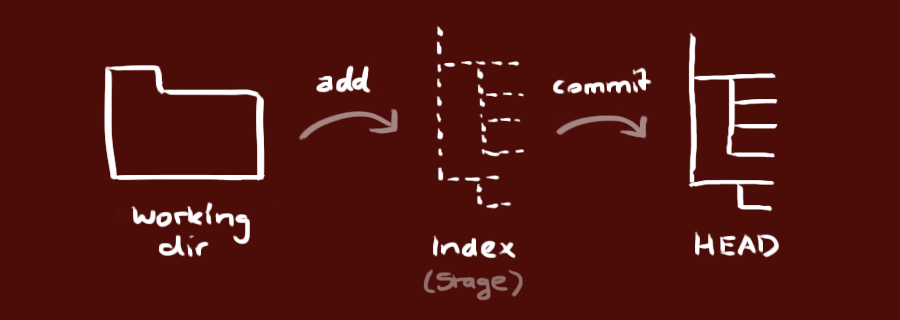
\includegraphics[width=\textwidth]{media/trees.png}
        \end{figure}
    \end{minipage}       
\end{frame}
\begin{frame}[fragile]{Primi comandi}
    Puoi proporre modifiche (aggiungendole all'Index cioè la lista dei file in attesa di commit) usando
    \begin{lstlisting}[language=bash]
$ git add <nomedelfile>
$ git add .
$ git add -p\end{lstlisting}
    Per togliere un file dalla staging area (senza perdere le modifiche) e per annullare le modifiche non ancora in stage:
    \begin{lstlisting}[language=bash]
$ git restore --staged <nomedelfile>
$ git restore <nomedelfile>\end{lstlisting}
    \lstinline{git rm <nomedelfile>} invece cancella il file e mette in stage la sua rimozione.

    Il secondo passo è creare un commit con le modifiche in stage:
    \begin{lstlisting}[language=bash]
$ git commit -m "Messaggio per il commit"\end{lstlisting}
\end{frame}
\begin{frame}[fragile]{Stato delle modifiche in corso}
    Per vedere lo stato delle modifiche in corso possiamo usare il comando 
    \begin{lstlisting}[language=bash]
$ git status\end{lstlisting}
    
    \begin{figure}
        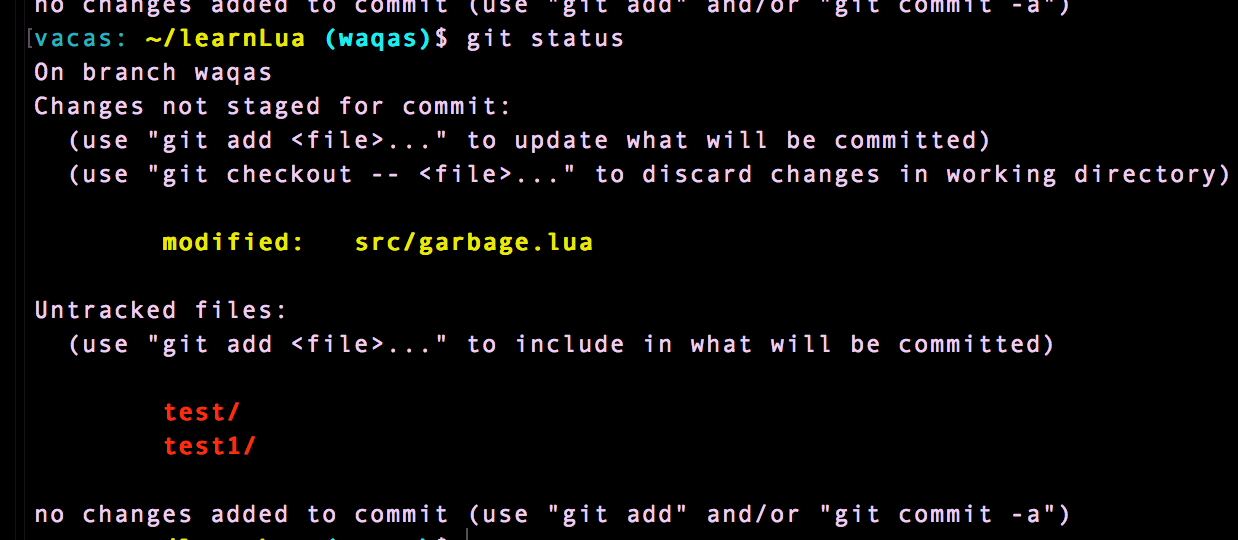
\includegraphics[width=0.55\textwidth]{media/git-status.png}
        
    \end{figure}
\end{frame}
\begin{frame}[fragile]{Lista dei commit}
    Per vedere la lista delle modifiche effettuate nel corso del tempo
    \begin{lstlisting}[language=bash]
$ git log\end{lstlisting}
    L'opzione \lstinline{--graph} mostra anche l'albero cronologico dei commit, molto utile nel caso di un repo con molti branch (\lstinline{git log --oneline --graph --all}).
    
    \begin{figure}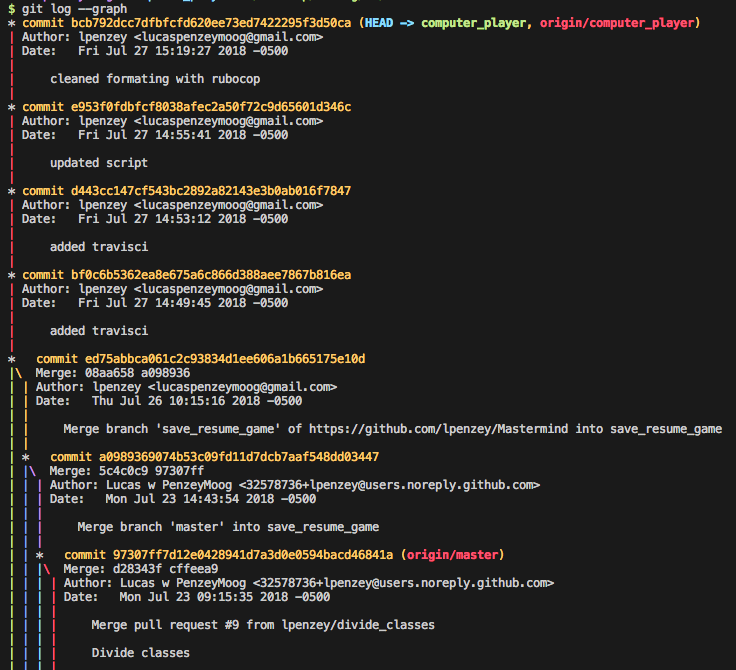
\includegraphics[width=0.55\textwidth,height=0.45\textheight,keepaspectratio]{media/git-log.png} \end{figure}
\end{frame}
\begin{frame}{Repository remoto}

    Abbiamo detto che Git utilizza un sistema di branching e merging per gestire le diverse linee di sviluppo, è bene sottolineare questo dettaglio in quanto tutte le operazioni di sincronizzazione del repository, sia in entrata che in uscita, sono legate a uno specifico branch.
    
    L'utente è libero di muoversi tra un branch e un altro nella working directory, e ogni branch locale può avere un upstream, cioè il branch del remote con cui si sincronizza.

    L'operazione di fetch serve anche per sincronizzare la lista dei remote branch.
\end{frame}
\begin{frame}[fragile]{Aggiungere un server remoto}
    Ora abbiamo committato le modifiche, che sono salvate in locale: non ci resta che sincronizzarle con il server remoto
    \begin{lstlisting}[language=bash]
$ git push <repo name> <branch name>
$ git push origin main\end{lstlisting}

    Se non hai clonato un repository esistente, ma ne hai creato uno nuovo e lo vuoi collegare a un server remoto, devi aggiungere il remote con:
    \begin{lstlisting}[language=bash]
$ git remote add origin <server>\end{lstlisting}
    Ora sarai in grado di inviare le tue modifiche al server remoto specificato

    Se non configurato, \lstinline{git init} crea ancora il branch \texttt{master}, mentre dal 2020 GitHub, GitLab e Bitbucket usano \texttt{main}. Conviene impostarlo una volta per tutte (o rinominare il branch corrente con \lstinline{git branch -M main}):
    \begin{lstlisting}[language=bash]
$ git config --global init.defaultBranch main\end{lstlisting}
\end{frame}
\begin{frame}[fragile]{Aggiorniamo il repo per vedere se ci sono modifiche e le scarichiamo}
    Per vedere se ci sono modifiche nel server remoto
    \begin{lstlisting}[language=bash]
$ git fetch\end{lstlisting}
    Per aggiornare il tuo repository locale al commit più recente, esegui
    \begin{lstlisting}[language=bash]
$ git pull\end{lstlisting}
    Se il branch locale e quello remoto sono divergenti, Git chiede di scegliere come integrarli: merge (\lstinline{git config --global pull.rebase false}) o rebase (\lstinline{git config --global pull.rebase true}).
\end{frame}
\begin{frame}[fragile]{Chi ha fatto cosa}
    Per sapere chi ha modificato per l'ultima volta ogni riga di un file possiamo utilizzare il comando
    \begin{lstlisting}[language=bash]
$ git blame README.MD\end{lstlisting}
    \lstinline{git blame} opera solamente su file singoli, è quindi richiesto il path di un file.
    L'opzione \lstinline{-M} rileva le linee spostate o copiate all'interno dello stesso file. In questo modo viene riportato l'autore originale delle righe invece dell'ultimo autore che ha spostato o copiato le righe.
    
    Il nome dal suono negativo deriva dal fatto che questo comando viene spesso usato per incolpare chi ha rotto un programma, anche se il suo utilizzo è molto più ampio.
    
    \begin{figure}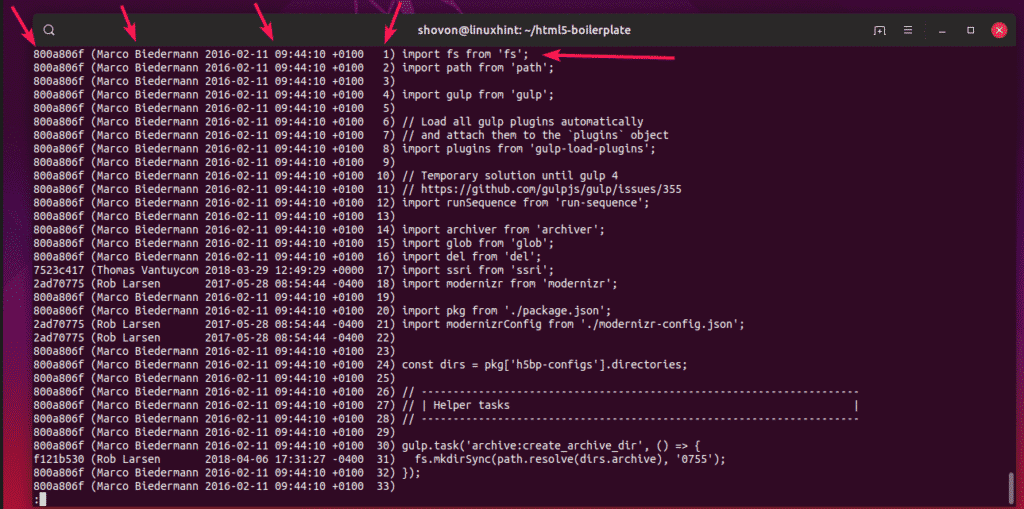
\includegraphics[width=0.55\textwidth,height=0.35\textheight,keepaspectratio]{media/git-blame.png} \end{figure}
    
\end{frame}
\begin{frame}{}\begin{figure}
    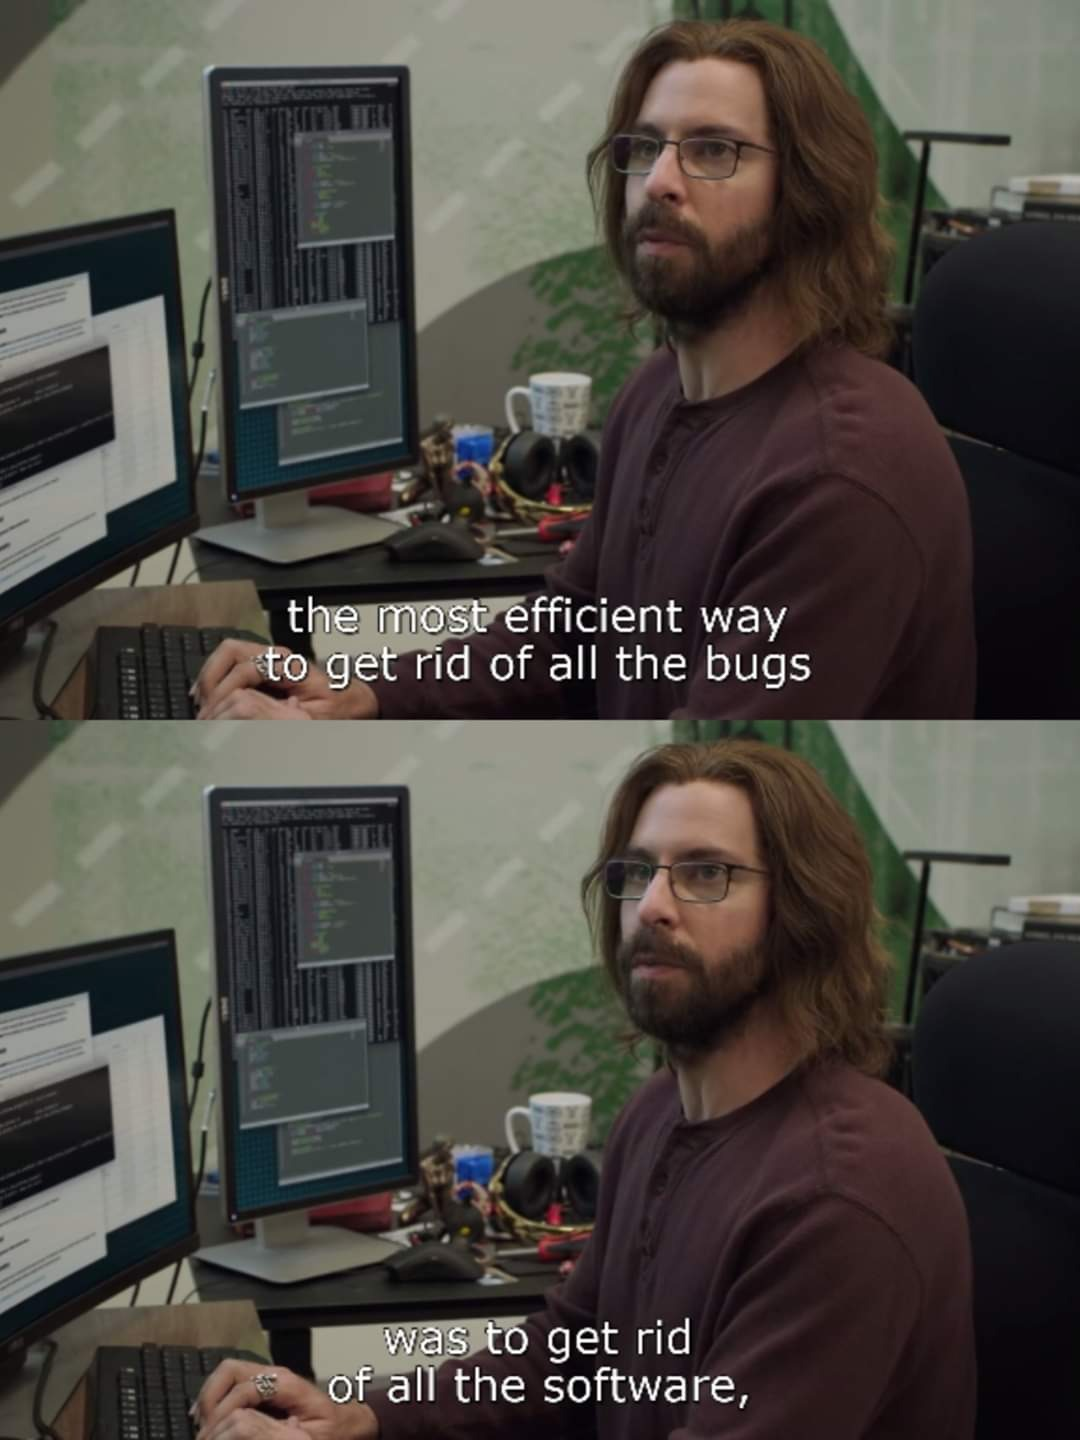
\includegraphics[height=0.95\textheight]{media/rid_of_all_the_sw.png} \end{figure}
\end{frame}
\begin{frame}{Sembra molto complicato rispetto a caricare i file su Dropbox}
    \begin{minipage}{0.47\textwidth}\begin{figure}
        
        
\includegraphics[width=1.0\textwidth]{media/meme-git.jpg} \end{figure}
    \end{minipage}
    \begin{minipage}{0.47\textwidth}
        Ecco, se usiamo servizi come Dropbox, Google Drive, OneDrive, Box, ... se troviamo un codice con tanti bug ci viene in mente di eliminarlo e non di correggerlo!
                        
        Inoltre l'utilizzo di Git (o software similari) è una routine in qualsiasi azienda di programmazione, meglio impararlo prima che dopo!
                        
        E ricordo: la history delle modifiche è importante e più utile di Ctrl+Z!
    \end{minipage}
\end{frame}
\begin{frame}{Procedure di sicurezza}
    \begin{figure}
        
        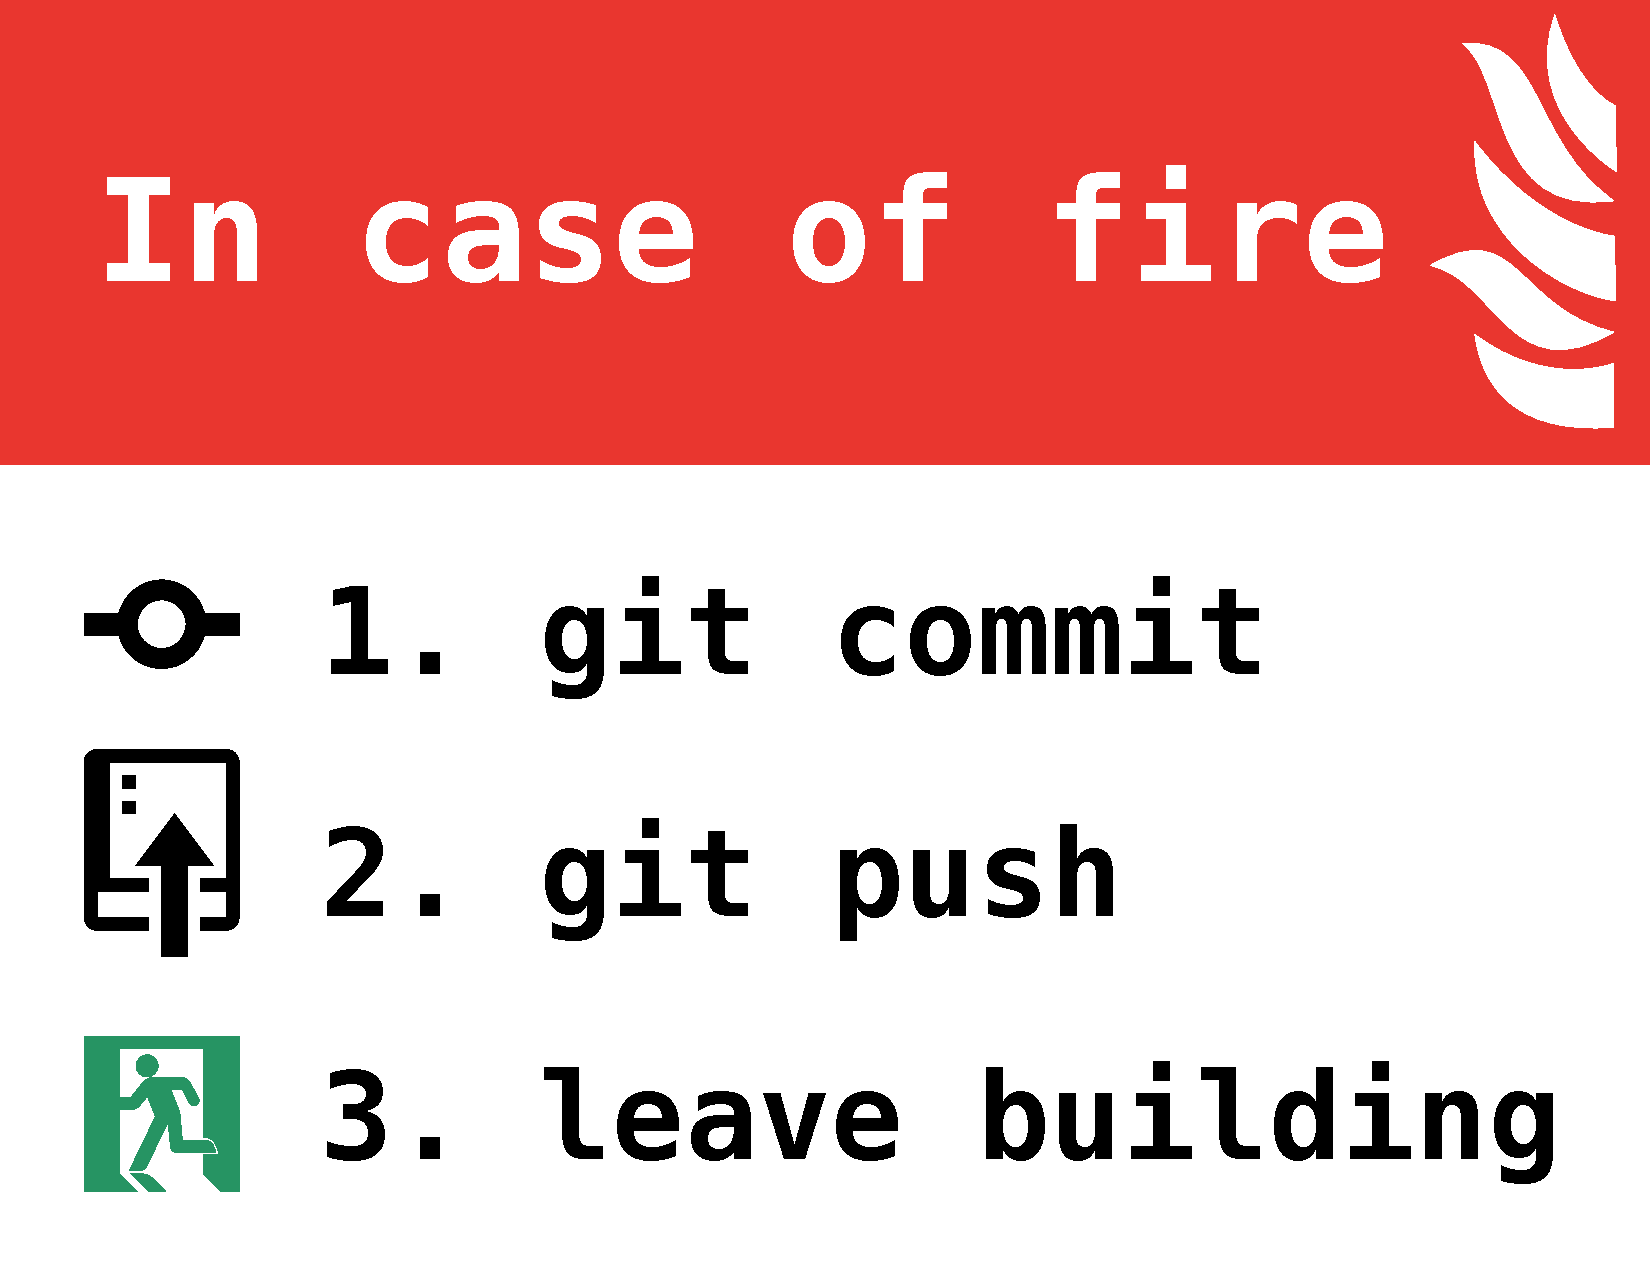
\includegraphics[width=0.5\textwidth]{media/in_case_of_fire.pdf}
    \end{figure}
    
\end{frame}

\section{Comandi di Git per il lavoro in gruppo}

\begin{frame}[fragile]{IDE \& .gitignore}
    È importante sottolineare che nel repository non ci vanno per nessun motivo i file compilati, i file di configurazione locali degli IDE e qualsiasi altra cosa legata al PC e non al progetto (soprattutto chiavi, token e password). Git mette a disposizione il file \texttt{.gitignore}, dove si specificano i file da ignorare. Una raccolta di template \texttt{.gitignore} è presente su questo repository:
    \url{https://github.com/github/gitignore}
    
    In linea generale, consiglio di unire in un solo file i template di JetBrains, Visual Studio, VS Code, Eclipse e quello del linguaggio di programmazione del repository (per esempio C++).
    
    Dopo aver modificato il file \texttt{.gitignore}, nel caso in cui nel nostro repository ci siano file la cui presenza non è gradita, possiamo usare questo comando per ``pulire'' il repository:
    \begin{lstlisting}[language=bash]
$ git rm -r --cached . 
$ git add .
$ git commit -am "Remove ignored files"\end{lstlisting}
\end{frame}
\begin{frame}{Workflow collaborativo}
    \begin{minipage}{0.5\textwidth}
        Quando si sviluppa in più persone si potrebbe pensare di tenere tutti i file su un server NAS e di modificarli lì, nessuna scelta è peggiore di questa: se uno sta facendo una modifica l'altro non può compilare e il NAS non gestisce modifiche contemporanee; ci sono altre soluzioni intermedie, sempre inadeguate. La soluzione è l'uso di un repository Git con più branch:
        \begin{itemize}
            \item \texttt{feature\_x} (con le tue modifiche)
            \item \texttt{feature\_y} (con le modifiche del collega)
            \item \texttt{dev} (o integrazione delle modifiche)
            \item \texttt{release} (o produzione)
        \end{itemize}
    \end{minipage} 
    \begin{minipage}{0.45\textwidth}
        Esempio di workflow collaborativo:
        \begin{figure}
            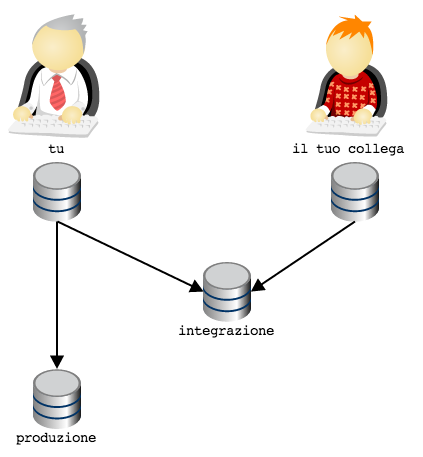
\includegraphics[width=0.6\textwidth]{media/workflow-5.png}
        \end{figure}
        Altri tip per ottimizzare il workflow (GitFlow, GitHub flow, trunk-based development): \url{https://get-git.readthedocs.io/it/latest/obiettivo_7.html}
    \end{minipage}
\end{frame} 
\begin{frame}{Fork}
    Con \textbf{Fork} si intende una determinata copia locale o remota di un repository ad uso e servizio di uno sviluppatore o di alcuni sviluppatori, e le modifiche vengono inviate alla copia principale tramite pull request. Pratica molto diffusa soprattutto nei progetti open source.
    \begin{figure}
        \scalebox{0.6}{
            \includegraphics[width=1.5\textwidth]{media/fork.tikz}
        }
    \end{figure}
\end{frame} 
\begin{frame}{Branching}
    Con \textbf{operazione di branching}, in quasi tutti i VCS, si intende l'operazione tramite la quale l'utente ``si stacca'' dal branch principale di sviluppo e continua a lavorare senza intaccarlo.
    In molti VCS è un'operazione dispendiosa in termini di risorse e tempo, e raramente fa parte del workflow.
    
    In Git invece il branching è diventato una parte vitale del workflow di lavoro di molti utenti grazie alla semplicità nel creare nuovi branch e spostarsi tra di essi.
    
    \begin{figure}
        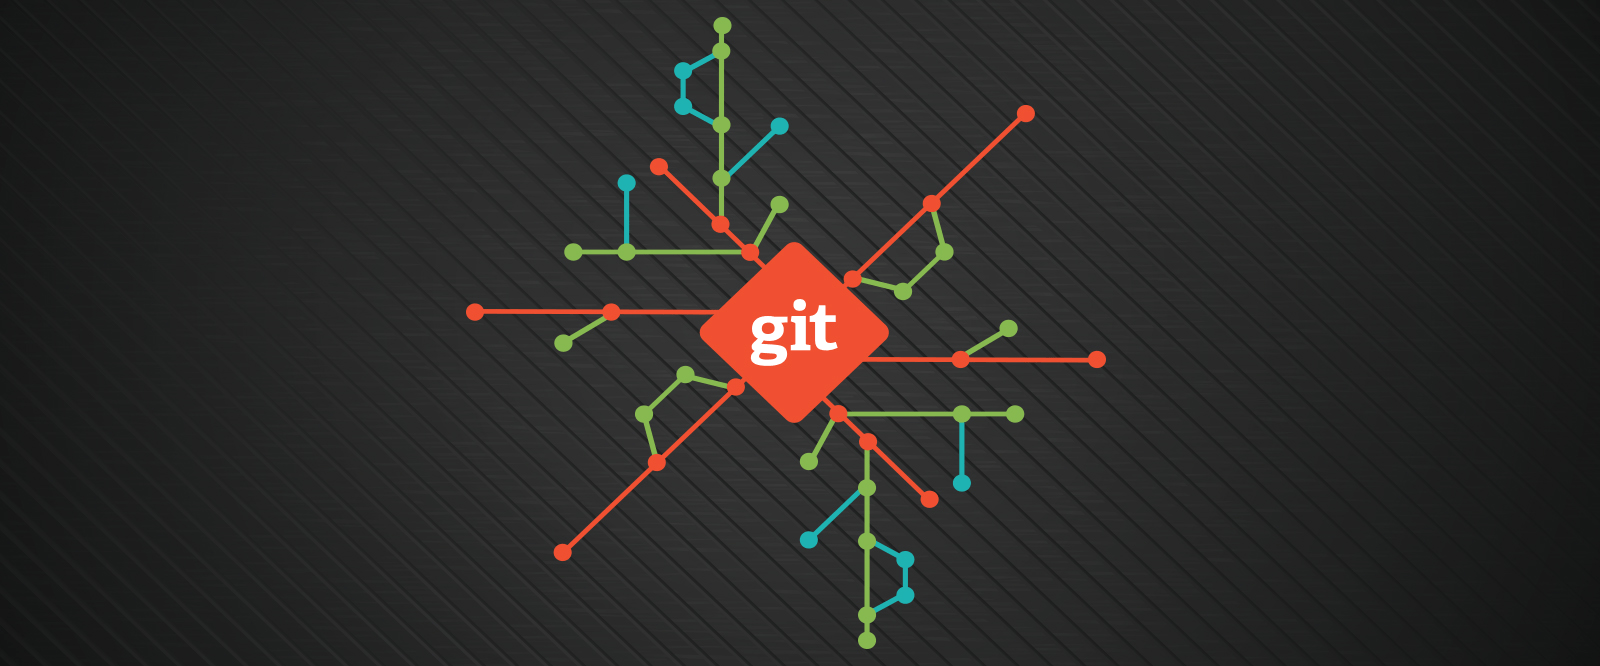
\includegraphics[width=0.5\textwidth]{media/git_branch.png}%
    \end{figure}
\end{frame}
\begin{frame}[fragile]{Branching}
    Crea un nuovo branch chiamato \texttt{feature\_x} e passa al nuovo branch usando
    \begin{lstlisting}[language=bash]
$ git switch -c feature_x\end{lstlisting}
    Ritorna di nuovo su \texttt{main}
    \begin{lstlisting}[language=bash]
$ git switch main\end{lstlisting}
    E, solamente dopo un merge, cancella il branch creato in precedenza
    \begin{lstlisting}[language=bash]
$ git branch -d feature_x\end{lstlisting}
    
    Il branch non sarà disponibile agli altri fino a quando non verrà inviato al repository remoto
    \begin{lstlisting}[language=bash]
$ git push origin <branch>\end{lstlisting}
    Con \lstinline{git push -u origin <branch>} diciamo a Git di impostare \texttt{origin/<branch>} come upstream, così la prossima volta basta scrivere:
\begin{lstlisting}[language=bash]
$ git push\end{lstlisting}
\end{frame}
\begin{frame}{Operazione di merge}
    Con operazione di merge, in tutti i VCS,  si intende
    l'operazione opposta del branching, tramite la quale si
    consolidano uno o più branch in un unico branch.
    
    \begin{figure}
        \scalebox{0.7}{
            \includegraphics{media/git-branch.tikz}
        }
    \end{figure}
\end{frame}
\begin{frame}[fragile]{Operazione di merge}{Scaricare ed unire le modifiche}
    Abbiamo visto che per aggiornare il tuo repository locale al commit più recente si esegue
    \begin{lstlisting}[language=bash]
$ git pull\end{lstlisting}
    Nella tua directory corrente per aggiornare il repository locale alla versione remota, in background il \texttt{git pull} effettua un \texttt{git fetch} e per incorporare le modifiche fatte sul server remoto effettua un \texttt{git merge} (o un \texttt{git rebase}, se configurato).
    Il comando pull cerca di auto-incorporare le modifiche locali con la copia nel server, ma questo non sempre è possibile. 
\end{frame}
\begin{frame}{Operazione di merge}{Scaricare ed unire le modifiche}    
    Il caso appena descritto è il caso banale di merge: cioè quello in cui il commit corrente è un antenato del commit con cui effettuiamo il merge: in questo caso si fa un merge fast-forward. Il riferimento del branch viene semplicemente spostato e viene eseguito il checkout del nuovo commit.

    \begin{figure}
        \includegraphics{media/merge-ff.tikz}
    \end{figure}

    Un altro caso banale è quello in cui il commit con cui effettuiamo il merge è un antenato del commit corrente. In questo caso non serve fare niente.
\end{frame}
\begin{frame}[fragile]{Operazione di Merge}{Effettuare il merge}
    Quando si devono unire invece le modifiche di un branch in un altro branch è necessario effettuare un merge a 3 vie e non il fast-forward. Per incorporare nel branch della working directory un altro branch (ad esempio \texttt{new-feature}):
    \begin{lstlisting}[language=bash]
$ git merge <branch>\end{lstlisting}

    La strategia di default, \texttt{ort} (da Git 2.34, prima \texttt{recursive}), prende il commit corrente (\texttt{ed489}), quello del branch da unire (\texttt{33a04}) e il loro antenato comune (\texttt{b325c}), ed esegue un merge a tre vie, creando un merge commit con due genitori (\texttt{f8bc5}).
    \vspace{-1em}
    \begin{figure}
        \includegraphics{media/merge.tikz}
    \end{figure}
\end{frame}
\begin{frame}[fragile]{Operazione di Merge}{Conflitti}
    L'algoritmo di Git riesce a effettuare senza problemi il merge di due branch se e solo se ogni parte di un file è stata modificata in al massimo uno dei due.

    In entrambi i casi Git prova ad auto-incorporare le modifiche. Sfortunatamente, a volte questa procedura automatizzata non è possibile, ed in questo caso ci saranno dei conflitti. 

    \begin{columns}
        \begin{column}{0.6\textwidth}
            Se invece la stessa parte di un file è stata modificata in entrambi, il merge si ferma e richiede un intervento manuale, riconoscibile da questi marker:
            \begin{lstlisting}
here is some content not affected by the conflict
<<<<<<< main
this is conflicted text from main
=======
this is conflicted text from feature branch
>>>>>>> feature\end{lstlisting}
        \end{column}
        \begin{column}{0.33\textwidth}
            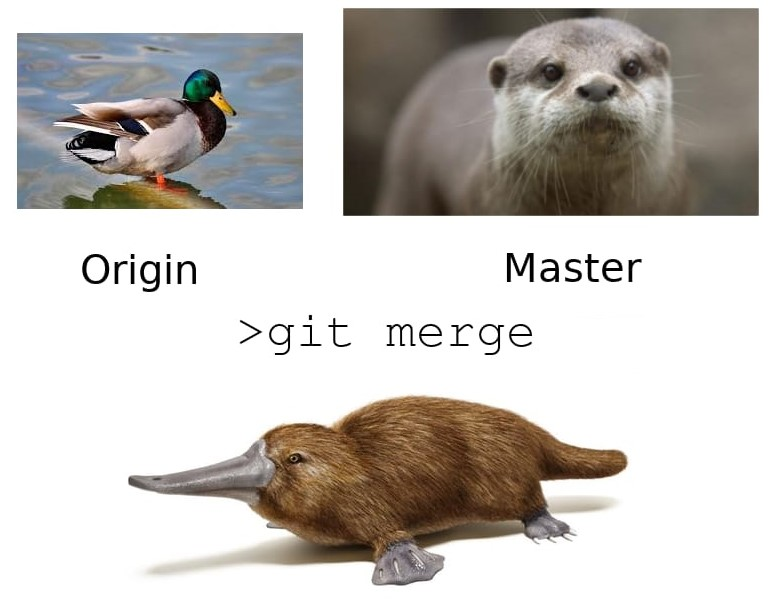
\includegraphics[width=\textwidth]{media/git-merge.jpeg}
        \end{column}
    \end{columns}
\end{frame}
\begin{frame}[fragile]{Operazione di Merge}{Conflitti}
    In caso di conflitti Git segna i file come ``unmerged'' (\lstinline{git status} li mostra come \texttt{both modified}).
    Una volta risolti i conflitti, si mettono i file in stage con:
    \begin{lstlisting}[language=bash]
$ git add <nomedelfile>\end{lstlisting}
    prima di fare il commit, puoi anche visualizzarne un'anteprima eseguendo
    \begin{lstlisting}[language=bash]
$ git diff <branch_sorgente> <branch_target>\end{lstlisting}
    Infine si effettua il commit (oppure si annulla tutto con \lstinline{git merge --abort}):
    \begin{lstlisting}[language=bash]
$ git commit\end{lstlisting}
\end{frame}
\begin{frame}[fragile]{Tags}
    È raccomandato creare dei tag quando il software viene rilasciato. È un concept già conosciuto, che esiste anche in SVN. Puoi creare un tag annotato chiamato v1.0.0 eseguendo
    \begin{lstlisting}[language=bash]
$ git tag -a v1.0.0 -m "Release 1.0.0" 1b2e1d63ff\end{lstlisting}
    la sequenza \texttt{1b2e1d63ff} rappresenta i primi 10 caratteri dell'hash del commit da taggare (si possono usare anche meno caratteri, basta che sia univoco), che puoi ottenere con \lstinline{git log}. Senza hash viene taggato il commit corrente.

    I tag non vengono inviati con il push normale:
    \begin{lstlisting}[language=bash]
$ git push origin v1.0.0\end{lstlisting}
\end{frame}
\begin{frame}[fragile]{Differenze apportate ai commit}
    Per Git, calcolare le modifiche apportate ai file da un commit all'altro non è poi difficile. Per esempio, puoi ricavarle con
    \begin{lstlisting}[language=bash]
$ git diff dev main\end{lstlisting}
    Con \lstinline{git diff from to} chiedi a Git «qual è l'elenco delle modifiche ai file che devo applicare a \texttt{from} perché il progetto diventi identico a quello fotografato in \texttt{to}»?
\end{frame}
\begin{frame}[fragile]{Cherry Pick}
    Con il comando \texttt{git cherry-pick} puoi chiedere a Git di calcolare le modifiche introdotte dal tuo commit e riapplicarle da qualche altra parte, per esempio, proprio su \texttt{main},  il nuovo commit ha lo stesso messaggio ma le modifiche sono applicate su un parent diverso.
    \begin{figure}
        \includegraphics{media/cherry-pick.tikz}
    \end{figure}
\end{frame}
\begin{frame}[fragile]{Merge con squash}
    Il comando \lstinline{git merge --squash} raggruppa tutti i commit in un unico commit con un unico genitore, come un cherry-pick dell'intero branch. Al termine il branch di lavoro si può cancellare.
    
    Supponiamo di avere un branch \texttt{new-feature} e di voler unire i vari commit in uno solo da aggiungere al branch \texttt{main}:
    \begin{lstlisting}[language=bash]
$ git merge --squash new-feature
$ git commit\end{lstlisting}
    \begin{figure}
        \includegraphics{media/merge-squash.tikz}
    \end{figure}
\end{frame}
\begin{frame}[fragile]{Rebase}
    Il comando \texttt{git rebase} permette di \textit{spostare} uno o più commit da un genitore all'altro, eseguendo un cherry-pick per tutti i commit presenti su un branch in un altro branch.
        
    A differenza di \texttt{git merge}, in cui si fa il merge nel branch principale, il rebase si fa sul branch secondario.

    In realtà i commit non vengono \textit{spostati}, in quanto  ogni commit è un oggetto unico e immutabile identificato in maniera univoca dal suo hash, ma viene creato un nuovo commit sulla base delle informazioni contenute nei vecchi oggetti (quindi rimangono le stesse informazioni, se non quella dei commit genitori e l'hash).

    \begin{figure}
        \scalebox{0.75}{
            \includegraphics{media/rebase.tikz}
        }
    \end{figure}
\end{frame}
\begin{frame}[fragile]{Rebase}
    Il comando precedente prende tutti i commit esistenti in topic ma non in main (precisamente \texttt{169a6}, \texttt{2c33a} e \texttt{3ba22}), li riapplica su main e poi sposta il branch sulla nuova estremità.
    
    Per limitare quanto andare all'indietro utilizzare l'opzione \lstinline{--onto}. Il comando seguente riporta sul main i commit più recenti del branch corrente da \texttt{169a6} (escluso), precisamente \texttt{2c33a} e \texttt{3ba22}.
    \begin{figure}
        \includegraphics{media/rebase-onto.tikz}
    \end{figure}
\end{frame}
\begin{frame}[fragile]{Rebase}{Git è (quasi) una blockchain}
    Esiste anche \lstinline{git rebase --interactive}, che permette di fare cose più complicate rispetto a riportare semplicemente commit, più precisamente eliminare, riordinare, modificare i commit.

    Ogni commit contiene l'hash dei genitori, quindi la history è una catena di hash (un Merkle DAG) come una blockchain. Nonostante ciò è possibile modificare e rimuovere i commit e riscrivere la history (ovviamente con nuovi hash, e poi serve un \lstinline{git push --force-with-lease}); per operazioni più complesse esistono \texttt{git filter-repo} e BFG Repo-Cleaner.
\end{frame}
\begin{frame}{Git \& DevOps}
    Attraverso un potente modello di branching e vari workflow
    di collaborazione, negli anni l'uso e l'adozione di Git è
    cresciuta esponenzialmente rispetto ad altri VCS, arrivando
    a essere il più usato e il più popolare, soprattutto perché è
    alla base di un processo DevOps: ogni push o pull request
    può avviare una pipeline di CI/CD (GitHub Actions, GitLab CI/CD,
    Bitbucket Pipelines) che compila, testa e rilascia il software.
\end{frame}

\section{Utilizzo di GitHub, GitLab e Bitbucket}

\begin{frame}{Utilizzo di GitHub, GitLab e Bitbucket}
    Questi sono alcuni servizi di hosting web-based per progetti che usano il sistema di controllo versione Git. Il primo è noto per l'hosting di moltissimi progetti open source, tra cui:
    \begin{enumerate}
        \item \url{https://github.com/torvalds/linux}
        \item \url{https://github.com/microsoft/MS-DOS} (ovviamente Git non c'era ai tempi dello sviluppo di MS-DOS e usavano i tasti CTRL+C e CTRL+V per fare lo storico delle versioni)
    \end{enumerate}
    GitLab e Bitbucket sono molto usati in ambito business, con numerosi servizi extra in cloud. Tutti e tre si possono installare on premise (GitHub Enterprise Server, GitLab Self-Managed, Bitbucket Data Center) e permettono la creazione di repository privati gratuiti.
    
\end{frame}

\begin{frame}[fragile]{Scarichiamo un repository da GitHub}
    Su GitHub troviamo il link (HTTPS o SSH) per scaricare il repository. Si noti che questo URL NON è l'URL della pagina web che si visita, ma l'URL che si trova con il pulsante ``Code''.
    \begin{figure} 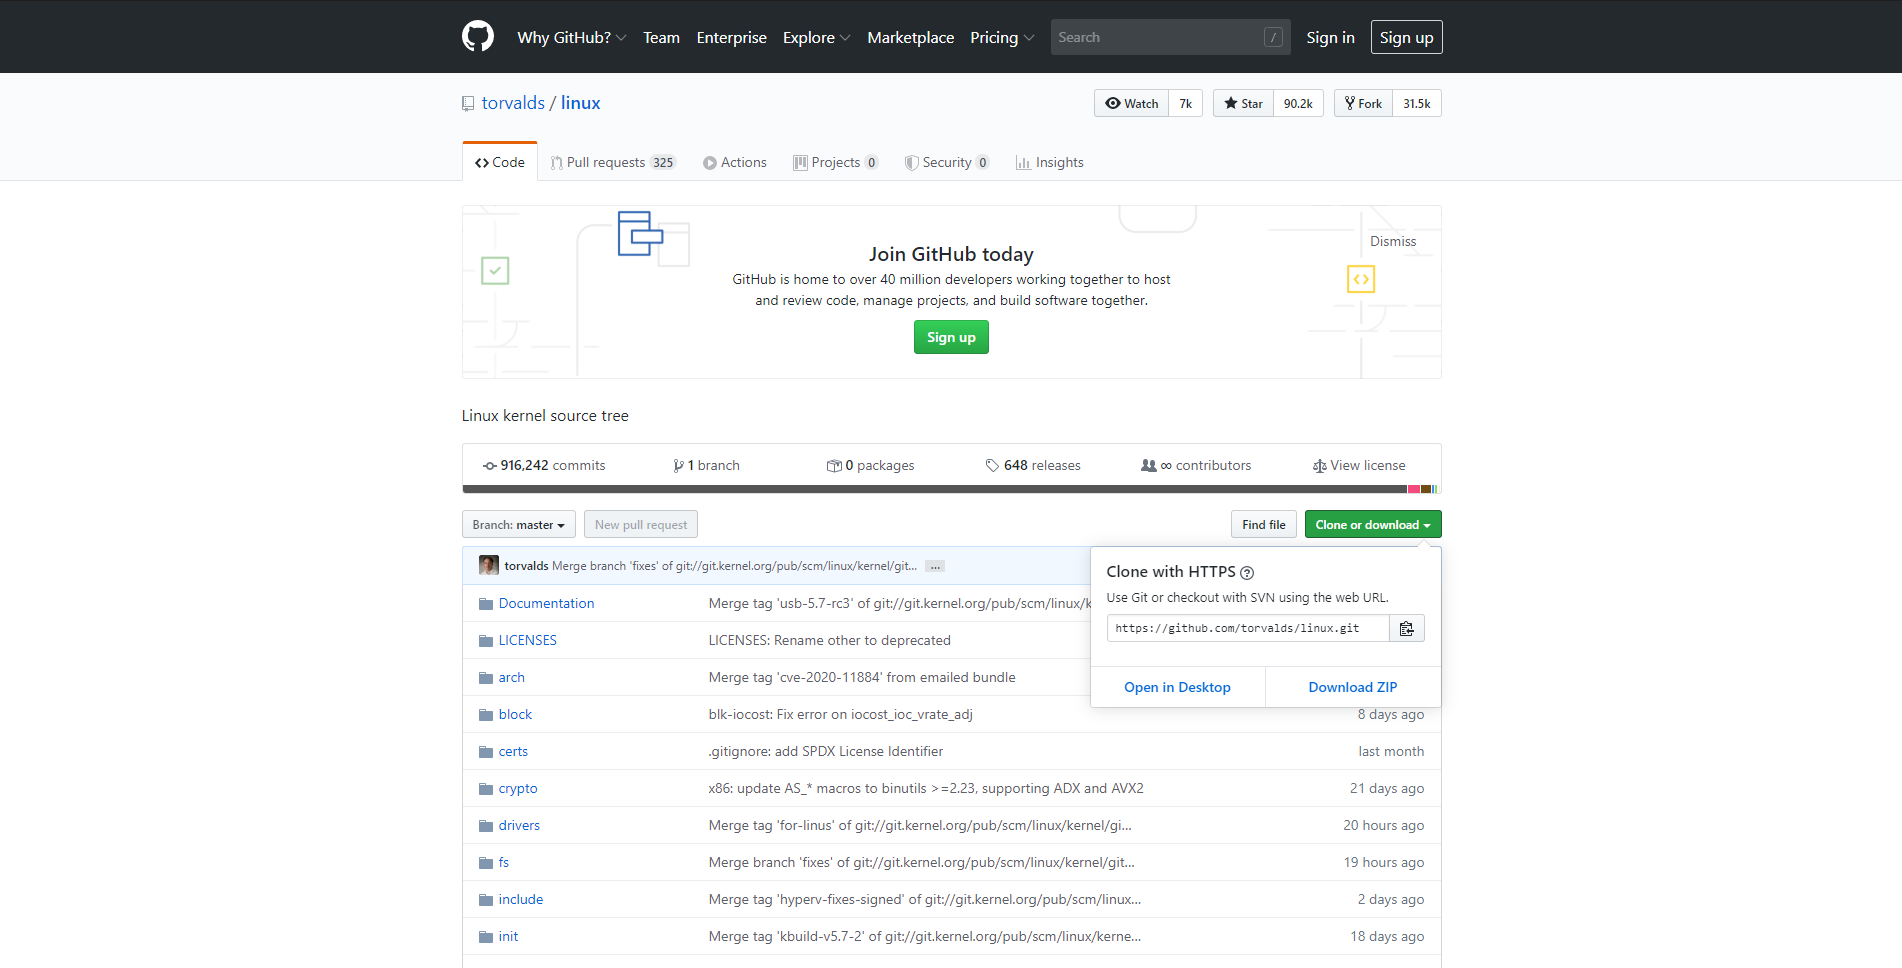
\includegraphics[width=0.6\textwidth]{media/github.PNG} \end{figure}
    
    \begin{lstlisting}[language=bash]
$ git clone git@github.com:user/test.git\end{lstlisting}
\end{frame}

\begin{frame}[fragile]{Utilizzo di GitLab}
    Creiamo un nuovo progetto su GitLab, dopo esserci registrati su GitLab (\url{https://gitlab.com/}), ricordo di usare una e-mail ``decente'' che possa identificare il programmatore e non furbissimo@gmail.com. Non stiamo scrivendo un software che hackera i server della NASA!
    
    Premiamo il pulsante ``New project'' e creiamo il nostro progetto. Diamogli un nome, per esempio ``test-GitLab'': dopo averlo creato ci appaiono delle semplici ``Command line instructions''. Le eseguiamo per esercitarci su Git. Una volta finito creiamo un file \texttt{.gitignore} e ``puliamo'' con i comandi il repository da eventuali file non ammessi!
    
    In maniera simile anche da GitLab un repo si scarica con \lstinline{git clone}. Si noti che questo URL NON è l'URL della pagina web che si visita, ma l'URL che si trova con il pulsante ``Code''.
    \begin{lstlisting}[language=bash]
$ git clone git@gitlab.com:gitlab-org/gitlab.git\end{lstlisting}
\end{frame}


\begin{frame}[fragile]{Utilizzo di Bitbucket}
    Come GitLab e GitHub, anche Bitbucket permette le stesse operazioni
    \begin{lstlisting}[language=bash]
$ git clone git@bitbucket.org:chromiumembedded/cef.git\end{lstlisting}
\end{frame}

\section{Git e JetBrains}

\begin{frame}{Git e JetBrains - Apertura di una repo}
    
    Una volta copiato il link al repo Git, se IntelliJ è aperto nella schermata di benvenuto è sufficiente cliccare su ``Clone Repository'' (nelle versioni precedenti ``Get from VCS''). Altrimenti, se un progetto è già aperto, si usa il menu ``Git'' \(\rightarrow\) ``Clone...''. Gli screenshot sono di una versione precedente dell'IDE, ma il flusso è lo stesso.
    
    
    \begin{columns}
        \begin{column}{0.5\textwidth}
            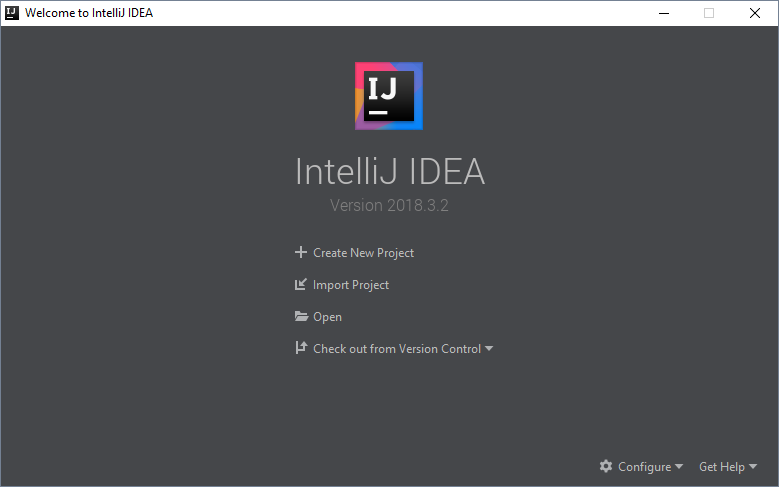
\includegraphics[width=\textwidth]{media/welcome.png}
        \end{column}
        \begin{column}{0.5\textwidth}
            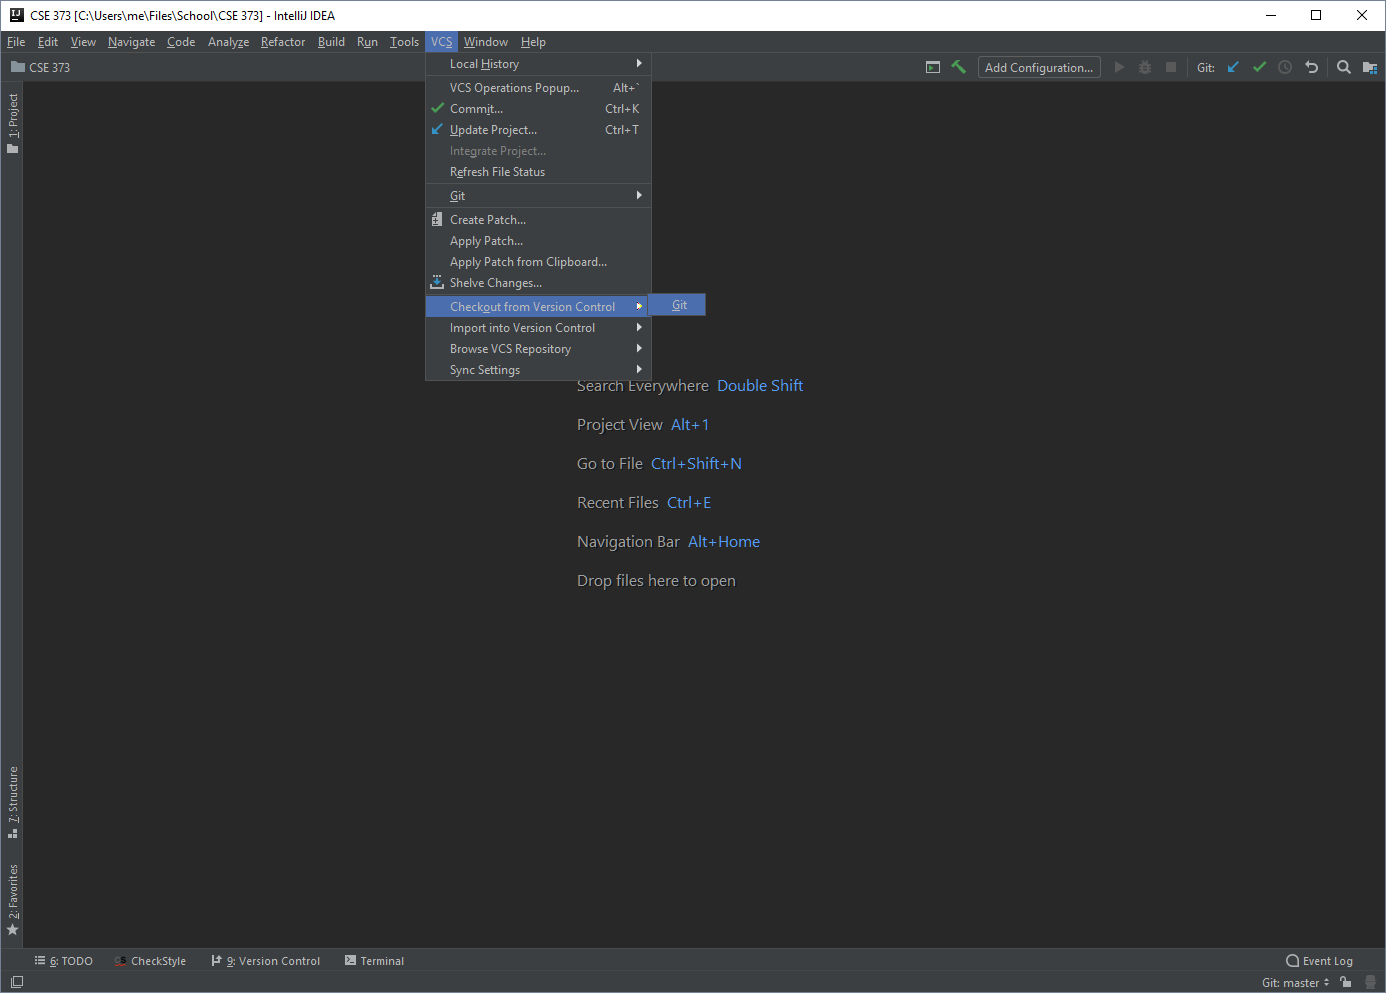
\includegraphics[width=\textwidth]{media/clone-menu.png}
            
        \end{column}
    \end{columns}
\end{frame}


\begin{frame}{Git e JetBrains - Apertura di una repo}
    In seguito si aprirà una finestra in cui inserire l'URL del repository che abbiamo copiato in precedenza (per esempio di GitLab, GitHub, ...) e una directory in cui salvare il repo clonato.
    
    \begin{figure} 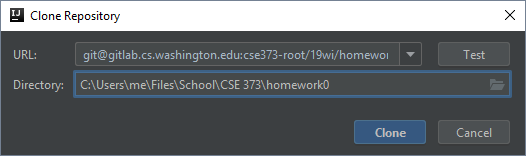
\includegraphics[width=0.3\textwidth]{media/clone-window.png} \end{figure}
    
    Se il clone è andato a buon fine, IntelliJ ti chiederà se vuoi aprire il progetto che hai appena clonato.
    
    \begin{figure} 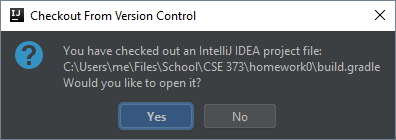
\includegraphics[width=0.3\textwidth]{media/clone-open.png} \end{figure}
    
    In linea generale bisogna premere Yes, ma ci sono alcuni casi in cui è meglio premere No.
    
\end{frame}

\begin{frame}{Git e JetBrains - Scaricare le modifiche}
    Prima di modificare un repo è bene scaricare le modifiche fatte nel frattempo dagli altri, per ridurre al minimo la possibilità di conflitti. Clicca ``Git'' \(\rightarrow\) ``Pull...'' e nella finestra che si apre premi ``Pull'' (oppure ``Update Project'', \keystroke{Ctrl}+\keystroke{T}).
    
    \begin{columns}
        \begin{column}{0.5\textwidth}
            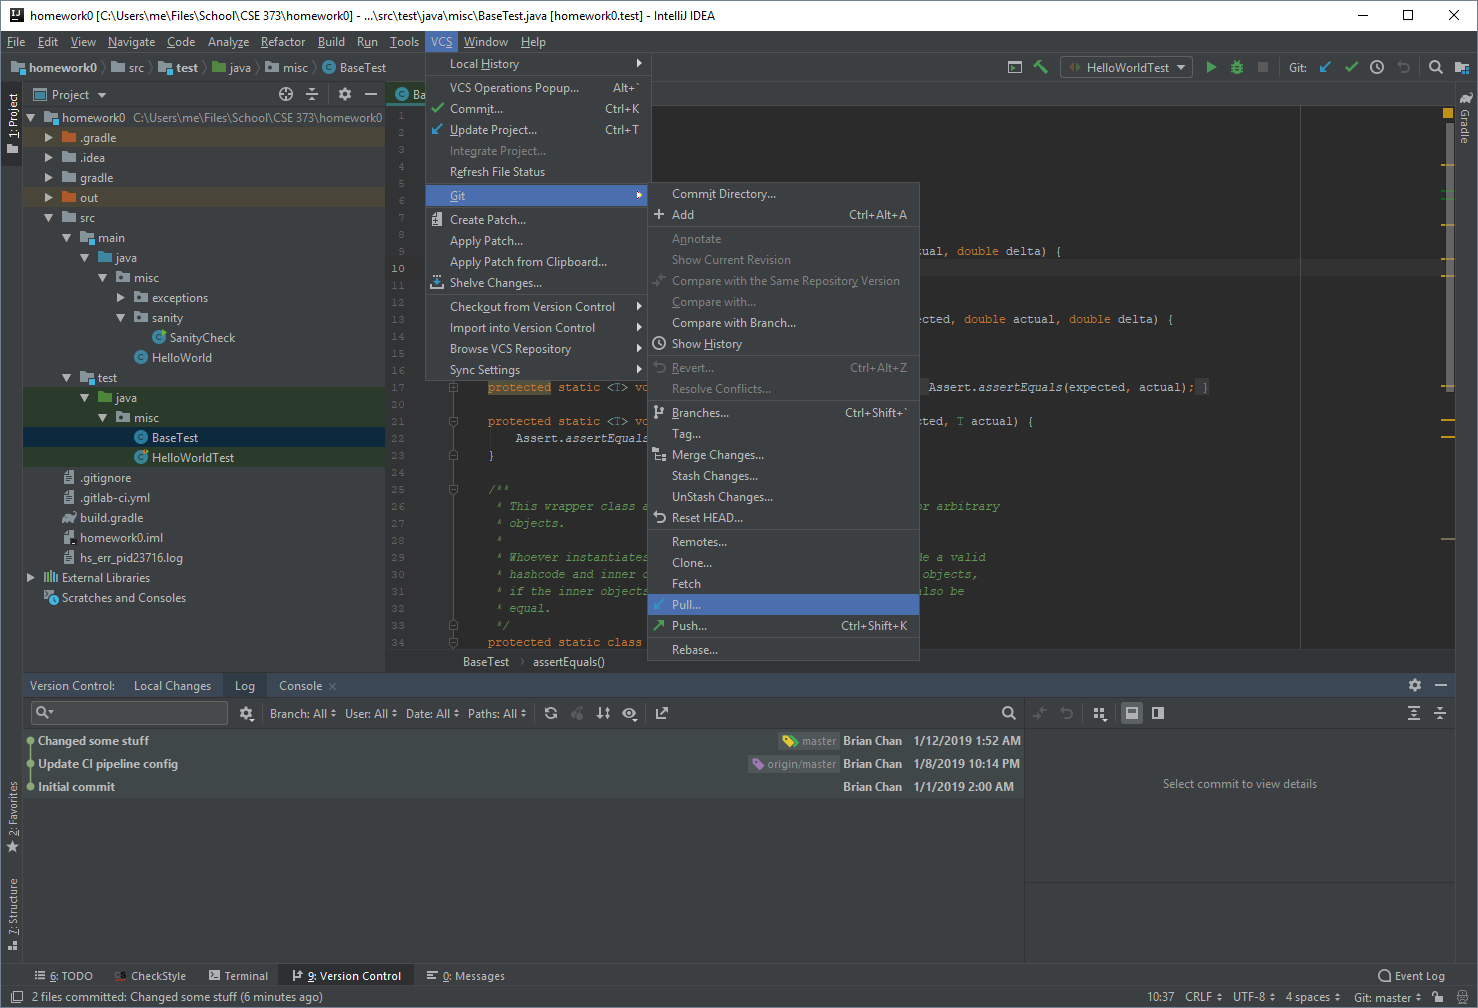
\includegraphics[width=\textwidth]{media/pull-menu.png}
        \end{column}
        \begin{column}{0.5\textwidth}
            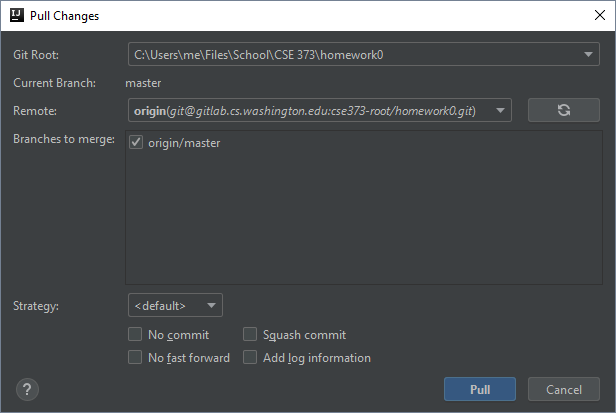
\includegraphics[width=\textwidth]{media/pull-window.png}
        \end{column}
    \end{columns}
    
    
\end{frame}

\begin{frame}{Git e JetBrains - Committare le modifiche}
    Una volta finite le modifiche apri la finestra di commit (``Git'' \(\rightarrow\) ``Commit...'', \keystroke{Ctrl}+\keystroke{K}). Seleziona i file da committare e aggiungi un commit message.
    \begin{figure} 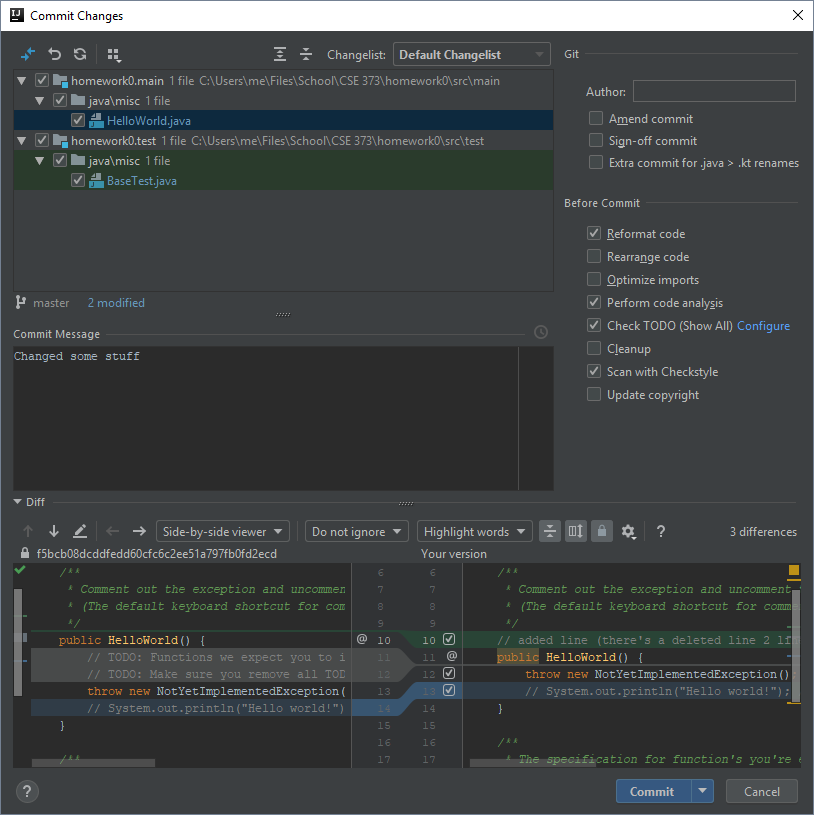
\includegraphics[width=0.35\textwidth]{media/commit.png} \end{figure}
    
\end{frame}


\begin{frame}{Git e JetBrains - Caricare le modifiche}
    Nella finestra precedente possiamo caricare subito le modifiche con ``Commit and Push'', ma non sempre è la cosa ideale (per esempio se siamo offline). Altrimenti apriamo la finestra ``Push'' dal menu ``Git'' \(\rightarrow\) ``Push...'' (\keystroke{Ctrl}+\keystroke{Shift}+\keystroke{K}).
    \begin{figure} 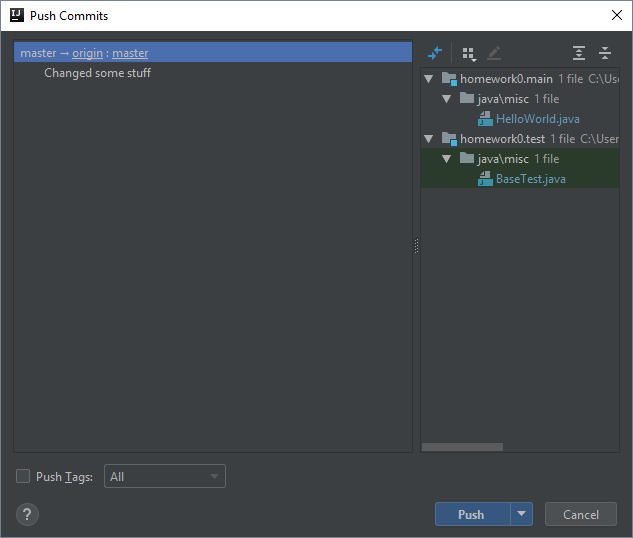
\includegraphics[width=0.35\textwidth]{media/push-window.png} \end{figure}
    
\end{frame}


\begin{frame}{Altre informazioni utili}
    
    Guida ufficiale su come utilizzare Git su IntelliJ: \url{https://www.jetbrains.com/help/idea/version-control-integration.html}

    Guida su come utilizzare Git su Visual Studio: \url{https://learn.microsoft.com/en-us/visualstudio/version-control/}

    Guida su come utilizzare Git su Visual Studio Code: \url{https://code.visualstudio.com/docs/sourcecontrol/overview}
    
\end{frame}
\section{Cosa non fa Git}

\begin{frame}[fragile]{Millennium Bug + 20}
    Si narra che negli anni 90 nel centro di calcolo UniPD, in via San Francesco 11, Padova. I tecnici avrebbero fixato il millennium bug shiftando di 20 anni le date (prassi assai comune) affinché il 1999 diventasse il 2019, caricando le modifiche in produzione con questo commit (Git all'epoca non esisteva, ma facciamo finta di sì):
    \begin{lstlisting}[language=bash]
$ git commit -m "sort of fixed mbug, we'll be fine for another 20 years"
$ git push\end{lstlisting}
    \begin{enumerate}
        \item Git non ti avvisa se hai fatto bug!
        \item Git non ha un'AI che si ricorda che fra 20 anni devi correggere un bug!
        \item Git è solamente un sistema di archiviazione del codice!
                
    \end{enumerate}
\end{frame}

\section{Collaborazione attraverso GitHub, GitLab e Bitbucket}
\begin{frame}{Collaborazione attraverso GitHub, GitLab e Bitbucket}
    In queste slide inizieremo esaminando come collaborare direttamente sui repository GitHub, GitLab e Bitbucket. Dedicheremo un po' di tempo ad approfondire la collaborazione tramite pull request e issue.
    
    
\end{frame}

\begin{frame}{Fork}
    Se vuoi contribuire direttamente a un progetto, devi esserne il proprietario o un collaboratore. Se vuoi contribuire ad un progetto open source che non possiedi e su cui non sei un collaboratore, dovrai farne una copia su GitHub/GitLab/bitbucket con il tuo account utente. Questo processo si chiama \textbf{fork}. Una volta fatto il fork di un progetto, sarai in grado di fare tutte le modifiche che vuoi al tuo fork (copia) e potrai richiedere che le tue modifiche vengano incorporate nel progetto originale usando una \textbf{pull request}. 
        
    I fork sono un buon modo per accettare i contributi di persone con cui non si lavora regolarmente, ma sono troppo scomodi per l'uso quotidiano in un team che lavora a stretto contatto. Per questo motivo, probabilmente vorrete collaborare direttamente su un unico repository.
    
    Tuttavia, è comunque importante utilizzare i branch e le pull request per mantenere il vostro lavoro separato.
\end{frame}

\begin{frame}{Pull request}
    Spesso nei repo si tiene il branch \texttt{main} protetto (branch protection), cioè modificabile solo tramite pull request, magari con review obbligatoria e CI verde. Su GitLab si chiamano \textbf{merge request}. Per crearne una si va nel tab ``Pull requests'' del repo e si clicca su ``New pull request'': a sinistra il branch base, a destra quello con le modifiche, poi ``Create pull request''. Se non ci sono conflitti si può fare il merge della pull request direttamente dal sito (merge commit, squash o rebase), altrimenti bisogna prima risolvere i conflitti.
        
    \begin{figure} 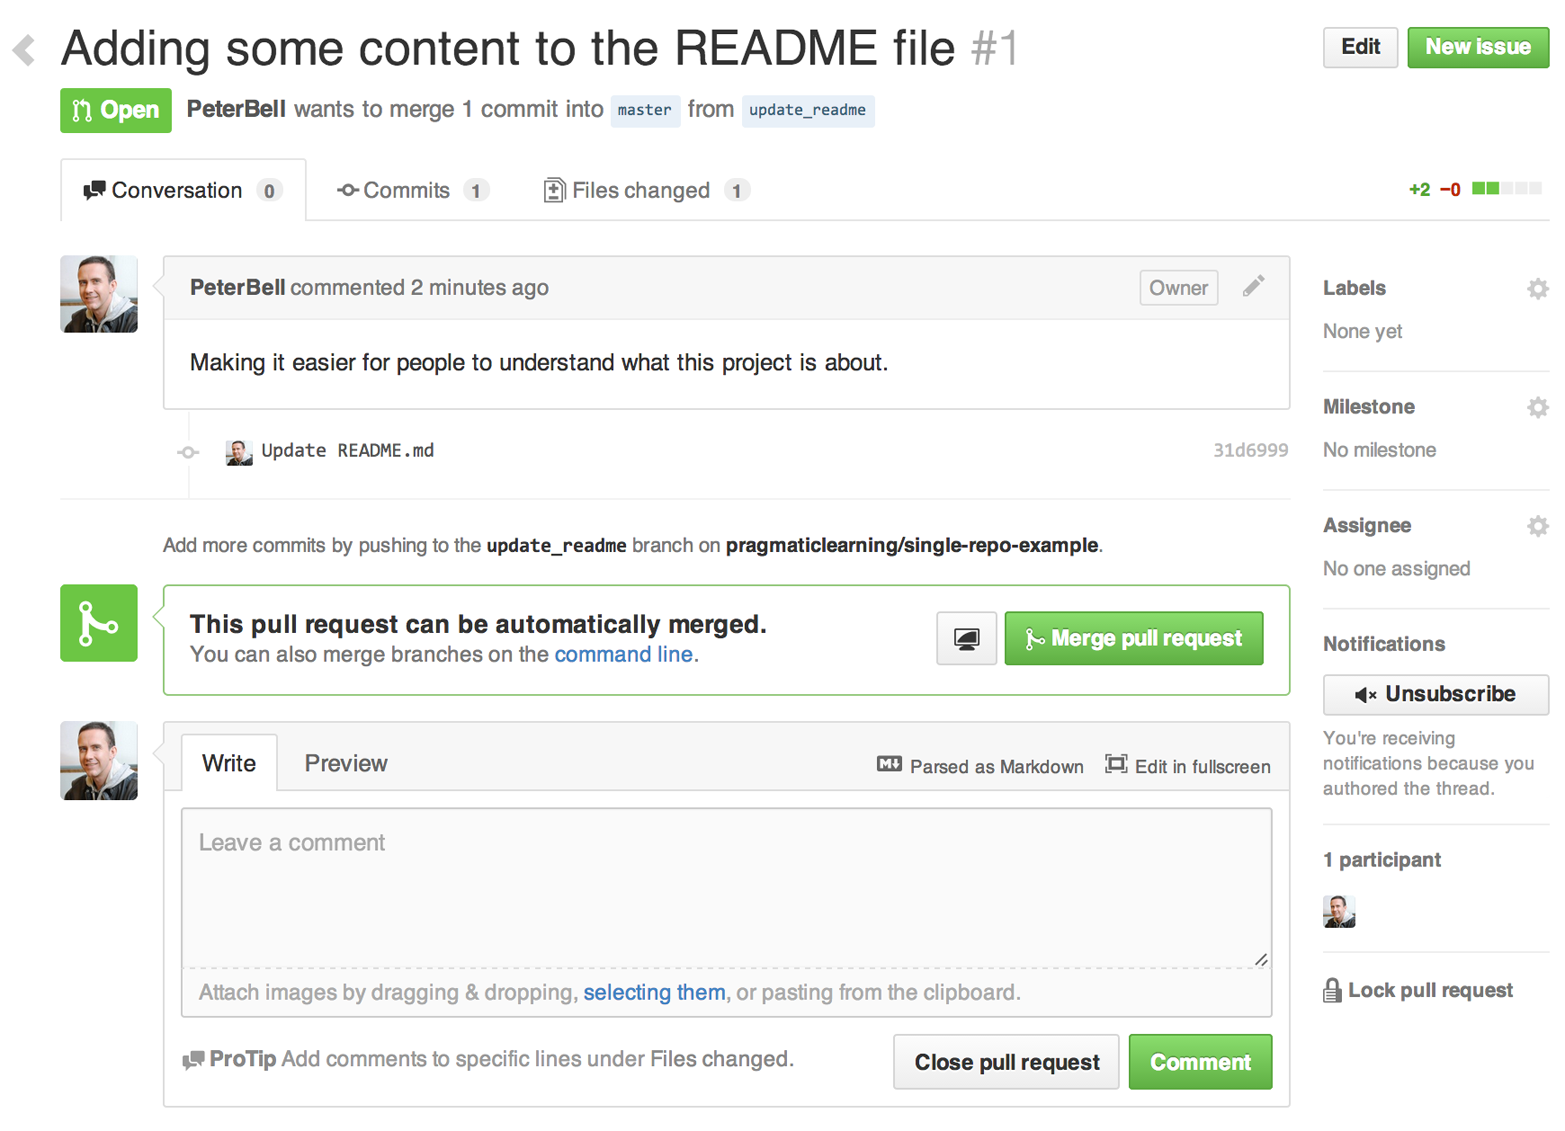
\includegraphics[width=0.5\textwidth,height=0.35\textheight,keepaspectratio]{media/pull-request.png} \end{figure}
    
        
    
\end{frame}

\begin{frame}
    {Issues}
    Un'ultima funzionalità degna di nota di GitHub, GitLab ecc. sono le Issues.
    
    Le Issues sono una bacheca condivisa da tutti gli sviluppatori dove vengono inseriti i bug e le feature mancanti, con titolo, descrizione e immagini. Permettono di assegnare ad ogni sviluppatore delle issue da risolvere e infine di chiuderle, anche in automatico da una pull request (``Fixes \#42'').
    \begin{columns}
        \begin{column}{0.5\textwidth}
            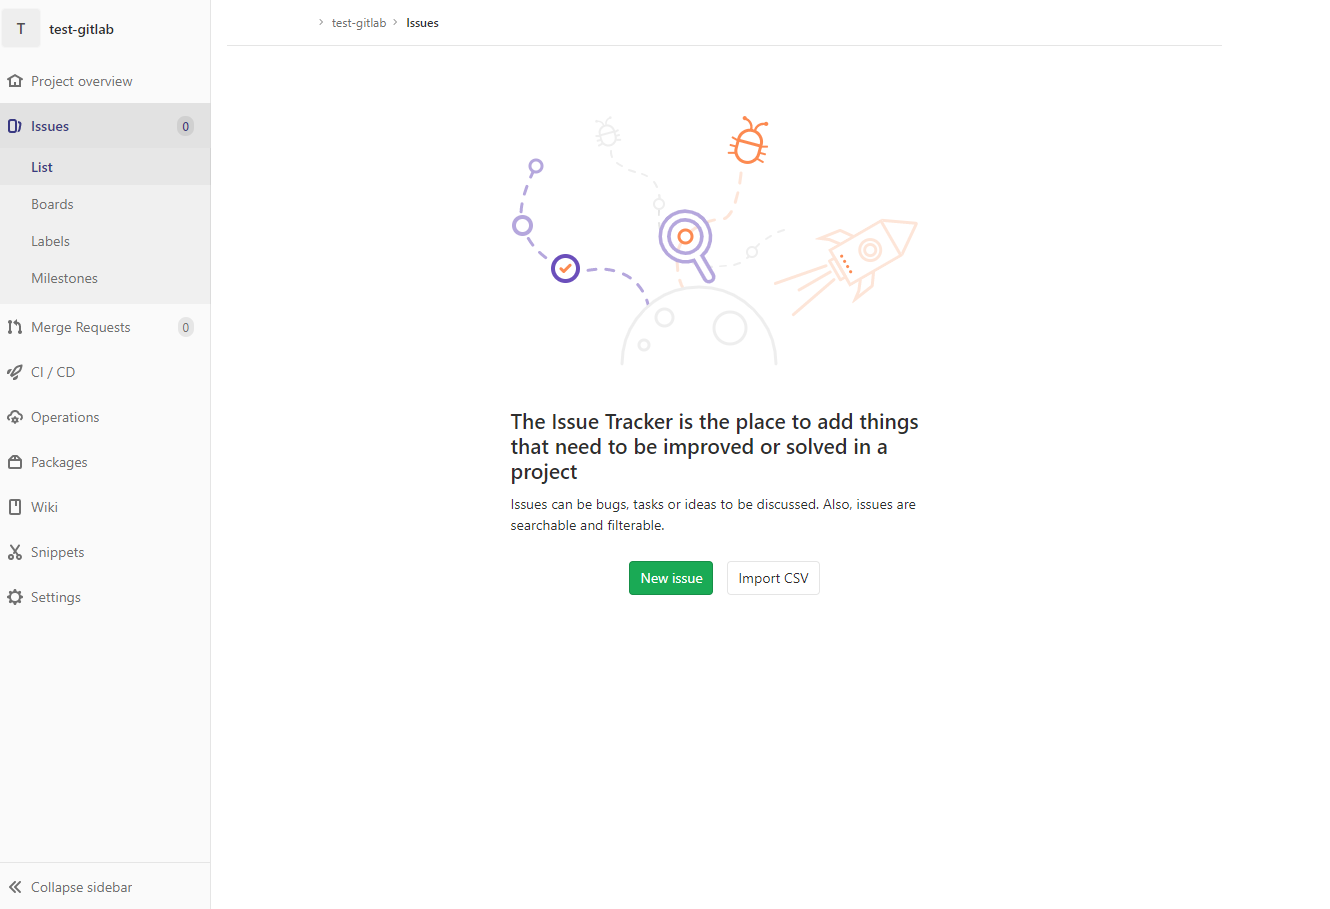
\includegraphics[width=\textwidth]{media/issues.png}
        \end{column}
        \begin{column}{0.5\textwidth}
            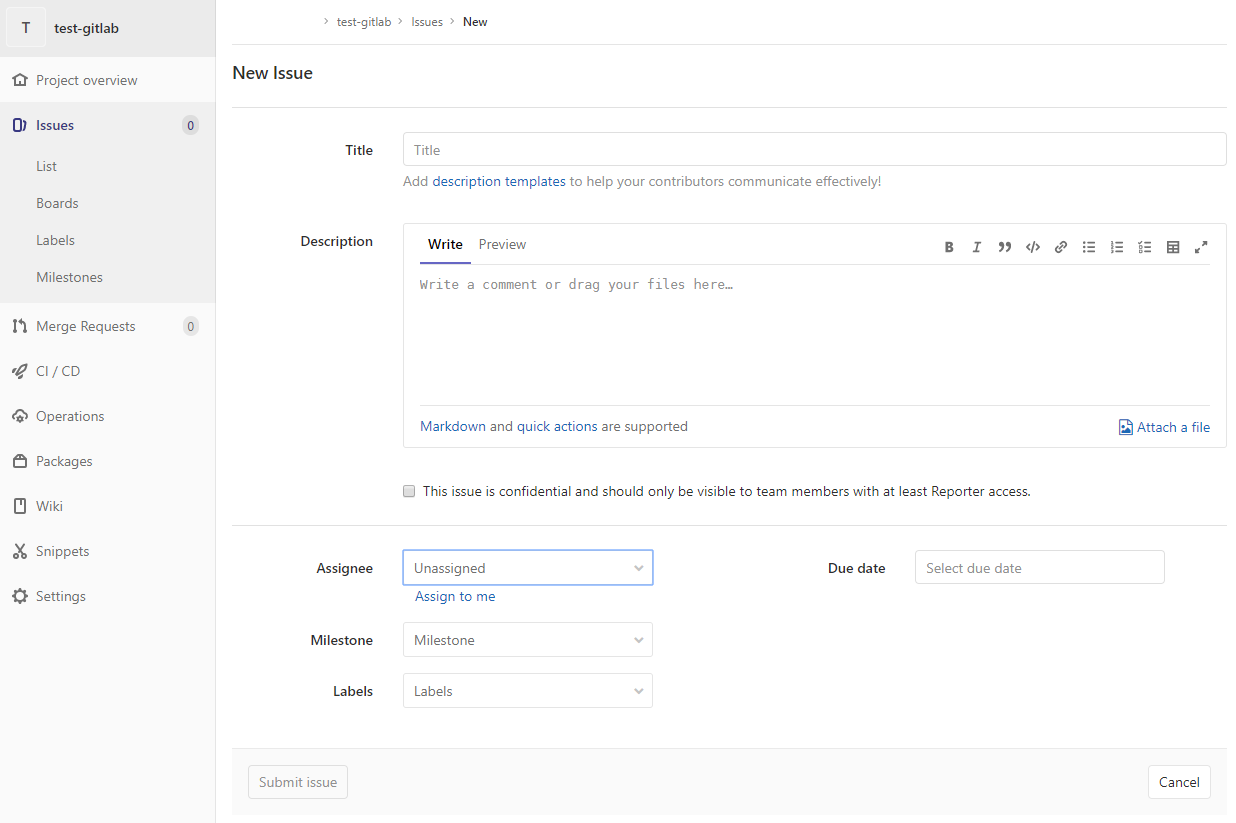
\includegraphics[width=\textwidth]{media/issuesA.png}
            
        \end{column}
    \end{columns}
\end{frame}

\begin{frame}{Come non usare gli Issues}
    \centering 
\includegraphics[width=0.8\textwidth]{media/issues.jpg}
    
    
\end{frame}

\begin{frame}{Fonti}
    \begin{itemize}
        \item Pro Git, 2\textsuperscript{a} edizione: \url{https://git-scm.com/book/it/v2}
        \item Documentazione di Git: \url{https://git-scm.com/docs}
        \item Credential helper: \url{https://git-scm.com/docs/gitcredentials}
        \item Git Credential Manager: \url{https://github.com/git-ecosystem/git-credential-manager}
        \item Strategie di merge (\texttt{ort}): \url{https://git-scm.com/docs/merge-strategies}
        \item Scalar: \url{https://git-scm.com/docs/scalar}
        \item Git LFS: \url{https://git-lfs.com/}
        \item \url{https://rogerdudler.github.io/git-guide/index.it.html}
        \item \url{https://www.atlassian.com/git/tutorials/setting-up-a-repository}
        \item \url{https://docs.github.com/en/get-started/git-basics/about-remote-repositories}
        \item \url{https://github.blog/news-insights/product-news/sunsetting-subversion-support/}
    \end{itemize}
\end{frame}
\begin{frame}{Fonti}
    \begin{itemize}
        \item \url{https://www.ionos.it/digitalguide/siti-web/programmazione-del-sito-web/git-vs-svn-controllo-di-versione-a-confronto/}
        \item \url{https://medium.com/@prasoon2211/mercurial-vs-git-scaling-and-architecture-94f70bb206ef}
        \item \url{https://www.mercurial-scm.org/wiki/Revlog}
        \item \url{https://github.com/microsoft/VFSForGit}
        \item Firma dei commit: \url{https://docs.github.com/en/authentication/managing-commit-signature-verification}
        \item \url{https://git-scm.com/book/en/v2/Git-Tools-Signing-Your-Work}
    \end{itemize}
\end{frame}
\end{document}